%**************************************%
%* Generated from MathBook XML source *%
%*    on 2016-09-01T15:21:19-05:00    *%
%*                                    *%
%*   http://mathbook.pugetsound.edu   *%
%*                                    *%
%**************************************%
\documentclass[10pt,]{book}
%% Load geometry package to allow page margin adjustments
\usepackage{geometry}
\geometry{letterpaper,total={5.0in,9.0in}}
%% Custom Preamble Entries, early (use latex.preamble.early)
%% Inline math delimiters, \(, \), need to be robust
%% 2016-01-31:  latexrelease.sty  supersedes  fixltx2e.sty
%% If  latexrelease.sty  exists, bugfix is in kernel
%% If not, bugfix is in  fixltx2e.sty
%% See:  https://tug.org/TUGboat/tb36-3/tb114ltnews22.pdf
%% and read "Fewer fragile commands" in distribution's  latexchanges.pdf
\IfFileExists{latexrelease.sty}{}{\usepackage{fixltx2e}}
%% Page Layout Adjustments (latex.geometry)
%% This LaTeX file may be compiled with pdflatex, xelatex, or lualatex
%% The following provides engine-specific capabilities
%% Generally, xelatex and lualatex will do better languages other than US English
%% You can pick from the conditional if you will only ever use one engine
\usepackage{ifthen}
\usepackage{ifxetex,ifluatex}
\ifthenelse{\boolean{xetex} \or \boolean{luatex}}{%
%% begin: xelatex and lualatex-specific configuration
%% fontspec package will make Latin Modern (lmodern) the default font
\ifxetex\usepackage{xltxtra}\fi
\usepackage{fontspec}
%% realscripts is the only part of xltxtra relevant to lualatex 
\ifluatex\usepackage{realscripts}\fi
%% 
%% Extensive support for other languages
\usepackage{polyglossia}
\setdefaultlanguage{english}
%% Magyar (Hungarian)
\setotherlanguage{magyar}
%% Spanish
\setotherlanguage{spanish}
%% Vietnamese
\setotherlanguage{vietnamese}
%% end: xelatex and lualatex-specific configuration
}{%
%% begin: pdflatex-specific configuration
%% translate common Unicode to their LaTeX equivalents
%% Also, fontenc with T1 makes CM-Super the default font
%% (\input{ix-utf8enc.dfu} from the "inputenx" package is possible addition (broken?)
\usepackage[T1]{fontenc}
\usepackage[utf8]{inputenc}
%% end: pdflatex-specific configuration
}
%% Monospace font: Inconsolata (zi4)
%% Sponsored by TUG: http://levien.com/type/myfonts/inconsolata.html
%% See package documentation for excellent instructions
%% One caveat, seem to need full file name to locate OTF files
%% Loads the "upquote" package as needed, so we don't have to
%% Upright quotes might come from the  textcomp  package, which we also use
%% We employ the shapely \ell to match Google Font version
%% pdflatex: "varqu" option produces best upright quotes
%% xelatex,lualatex: add StylisticSet 1 for shapely \ell
%% xelatex,lualatex: add StylisticSet 2 for plain zero
%% xelatex,lualatex: we add StylisticSet 3 for upright quotes
%% 
\ifthenelse{\boolean{xetex} \or \boolean{luatex}}{%
%% begin: xelatex and lualatex-specific monospace font
\usepackage{zi4}
\setmonofont[BoldFont=Inconsolatazi4-Bold.otf,StylisticSet={1,3}]{Inconsolatazi4-Regular.otf}
%% end: xelatex and lualatex-specific monospace font
}{%
%% begin: pdflatex-specific monospace font
\usepackage[varqu]{zi4}
%% end: pdflatex-specific monospace font
}
%% Symbols, align environment, bracket-matrix
\usepackage{amsmath}
\usepackage{amssymb}
%% allow more columns to a matrix
%% can make this even bigger by overriding with  latex.preamble.late  processing option
\setcounter{MaxMatrixCols}{30}
%%
%% Color support, xcolor package
%% Always loaded.  Used for:
%% mdframed boxes, add/delete text, author tools
\PassOptionsToPackage{usenames,dvipsnames,svgnames,table}{xcolor}
\usepackage{xcolor}
%%
%% Semantic Macros
%% To preserve meaning in a LaTeX file
%% Only defined here if required in this document
%% Subdivision Numbering, Chapters, Sections, Subsections, etc
%% Subdivision numbers may be turned off at some level ("depth")
%% A section *always* has depth 1, contrary to us counting from the document root
%% The latex default is 3.  If a larger number is present here, then
%% removing this command may make some cross-references ambiguous
%% The precursor variable $numbering-maxlevel is checked for consistency in the common XSL file
\setcounter{secnumdepth}{3}
%% Environments with amsthm package
%% Theorem-like environments in "plain" style, with or without proof
\usepackage{amsthm}
\theoremstyle{plain}
%% Numbering for Theorems, Conjectures, Examples, Figures, etc
%% Controlled by  numbering.theorems.level  processing parameter
%% Always need a theorem environment to set base numbering scheme
%% even if document has no theorems (but has other environments)
\newtheorem{theorem}{Theorem}[section]
%% Only variants actually used in document appear here
%% Style is like a theorem, and for statements without proofs
%% Numbering: all theorem-like numbered consecutively
%% i.e. Corollary 4.3 follows Theorem 4.2
\newtheorem{corollary}[theorem]{Corollary}
%% Definition-like environments, normal text
%% Numbering is in sync with theorems, etc
\theoremstyle{definition}
\newtheorem{definition}[theorem]{Definition}
%% Example-like environments, normal text
%% Numbering is in sync with theorems, etc
\theoremstyle{definition}
\newtheorem{example}[theorem]{Example}
%% Localize LaTeX supplied names (possibly none)
\renewcommand*{\proofname}{Proof}
\renewcommand*{\chaptername}{Chapter}
%% Equation Numbering
%% Controlled by  numbering.equations.level  processing parameter
\numberwithin{equation}{section}
%% For improved tables
\usepackage{array}
%% Some extra height on each row is desirable, especially with horizontal rules
%% Increment determined experimentally
\setlength{\extrarowheight}{0.2ex}
%% Define variable thickness horizontal rules, full and partial
%% Thicknesses are 0.03, 0.05, 0.08 in the  booktabs  package
\makeatletter
\newcommand{\hrulethin}  {\noalign{\hrule height 0.04em}}
\newcommand{\hrulemedium}{\noalign{\hrule height 0.07em}}
\newcommand{\hrulethick} {\noalign{\hrule height 0.11em}}
%% We preserve a copy of the \setlength package before other
%% packages (extpfeil) get a chance to load packages that redefine it
\let\oldsetlength\setlength
\newlength{\Oldarrayrulewidth}
\newcommand{\crulethin}[1]%
{\noalign{\global\oldsetlength{\Oldarrayrulewidth}{\arrayrulewidth}}%
\noalign{\global\oldsetlength{\arrayrulewidth}{0.04em}}\cline{#1}%
\noalign{\global\oldsetlength{\arrayrulewidth}{\Oldarrayrulewidth}}}%
\newcommand{\crulemedium}[1]%
{\noalign{\global\oldsetlength{\Oldarrayrulewidth}{\arrayrulewidth}}%
\noalign{\global\oldsetlength{\arrayrulewidth}{0.07em}}\cline{#1}%
\noalign{\global\oldsetlength{\arrayrulewidth}{\Oldarrayrulewidth}}}
\newcommand{\crulethick}[1]%
{\noalign{\global\oldsetlength{\Oldarrayrulewidth}{\arrayrulewidth}}%
\noalign{\global\oldsetlength{\arrayrulewidth}{0.11em}}\cline{#1}%
\noalign{\global\oldsetlength{\arrayrulewidth}{\Oldarrayrulewidth}}}
%% Single letter column specifiers defined via array package
\newcolumntype{A}{!{\vrule width 0.04em}}
\newcolumntype{B}{!{\vrule width 0.07em}}
\newcolumntype{C}{!{\vrule width 0.11em}}
\makeatother
%% Figures, Tables, Listings, Floats
%% The [H]ere option of the float package fixes floats in-place,
%% in deference to web usage, where floats are totally irrelevant
%% We re/define the figure, table and listing environments, if used
%%   1) New mbxfigure and/or mbxtable environments are defined with float package
%%   2) Standard LaTeX environments redefined to use new environments
%%   3) Standard LaTeX environments redefined to step theorem counter
%%   4) Counter for new environments is set to the theorem counter before caption
%% You can remove all this figure/table setup, to restore standard LaTeX behavior
%% HOWEVER, numbering of figures/tables AND theorems/examples/remarks, etc
%% WILL ALL de-synchronize with the numbering in the HTML version
%% You can remove the [H] argument of the \newfloat command, to allow flotation and 
%% preserve numbering, BUT the numbering may then appear "out-of-order"
\usepackage{float}
\usepackage[bf]{caption} % http://tex.stackexchange.com/questions/95631/defining-a-new-type-of-floating-environment 
\usepackage{newfloat}
% Table environment setup so that it no longer floats
\SetupFloatingEnvironment{table}{fileext=lot,placement={H},within=section,name=Table}
% tables have the same number as theorems: http://tex.stackexchange.com/questions/16195/how-to-make-equations-figures-and-theorems-use-the-same-numbering-scheme 
\makeatletter
\let\c@table\c@theorem
\makeatother
%% Raster graphics inclusion, wrapped figures in paragraphs
%% \resizebox sometimes used for images in side-by-side layout
\usepackage{graphicx}
%%
%% Program listing support, for inline code, Sage code
\usepackage{listings}
%% We define the listings font style to be the default "ttfamily"
%% To fix hyphens/dashes rendered in PDF as fancy minus signs by listing
%% http://tex.stackexchange.com/questions/33185/listings-package-changes-hyphens-to-minus-signs
\makeatletter
\lst@CCPutMacro\lst@ProcessOther {"2D}{\lst@ttfamily{-{}}{-{}}}
\@empty\z@\@empty
\makeatother
\ifthenelse{\boolean{xetex}}{}{%
%% begin: pdflatex-specific listings configuration
%% translate U+0080 - U+00F0 to their textmode LaTeX equivalents
%% Data originally from https://www.w3.org/Math/characters/unicode.xml, 2016-07-23
%% Lines marked in XSL with "$" were converted from mathmode to textmode
\lstset{extendedchars=true}
\lstset{literate={ }{{~}}{1}{¡}{{\textexclamdown }}{1}{¢}{{\textcent }}{1}{£}{{\textsterling }}{1}{¤}{{\textcurrency }}{1}{¥}{{\textyen }}{1}{¦}{{\textbrokenbar }}{1}{§}{{\textsection }}{1}{¨}{{\textasciidieresis }}{1}{©}{{\textcopyright }}{1}{ª}{{\textordfeminine }}{1}{«}{{\guillemotleft }}{1}{¬}{{\textlnot }}{1}{­}{{\-}}{1}{®}{{\textregistered }}{1}{¯}{{\textasciimacron }}{1}{°}{{\textdegree }}{1}{±}{{\textpm }}{1}{²}{{\texttwosuperior }}{1}{³}{{\textthreesuperior }}{1}{´}{{\textasciiacute }}{1}{µ}{{\textmu }}{1}{¶}{{\textparagraph }}{1}{·}{{\textperiodcentered }}{1}{¸}{{\c{}}}{1}{¹}{{\textonesuperior }}{1}{º}{{\textordmasculine }}{1}{»}{{\guillemotright }}{1}{¼}{{\textonequarter }}{1}{½}{{\textonehalf }}{1}{¾}{{\textthreequarters }}{1}{¿}{{\textquestiondown }}{1}{À}{{\`{A}}}{1}{Á}{{\'{A}}}{1}{Â}{{\^{A}}}{1}{Ã}{{\~{A}}}{1}{Ä}{{\"{A}}}{1}{Å}{{\AA }}{1}{Æ}{{\AE }}{1}{Ç}{{\c{C}}}{1}{È}{{\`{E}}}{1}{É}{{\'{E}}}{1}{Ê}{{\^{E}}}{1}{Ë}{{\"{E}}}{1}{Ì}{{\`{I}}}{1}{Í}{{\'{I}}}{1}{Î}{{\^{I}}}{1}{Ï}{{\"{I}}}{1}{Ð}{{\DH }}{1}{Ñ}{{\~{N}}}{1}{Ò}{{\`{O}}}{1}{Ó}{{\'{O}}}{1}{Ô}{{\^{O}}}{1}{Õ}{{\~{O}}}{1}{Ö}{{\"{O}}}{1}{×}{{\texttimes }}{1}{Ø}{{\O }}{1}{Ù}{{\`{U}}}{1}{Ú}{{\'{U}}}{1}{Û}{{\^{U}}}{1}{Ü}{{\"{U}}}{1}{Ý}{{\'{Y}}}{1}{Þ}{{\TH }}{1}{ß}{{\ss }}{1}{à}{{\`{a}}}{1}{á}{{\'{a}}}{1}{â}{{\^{a}}}{1}{ã}{{\~{a}}}{1}{ä}{{\"{a}}}{1}{å}{{\aa }}{1}{æ}{{\ae }}{1}{ç}{{\c{c}}}{1}{è}{{\`{e}}}{1}{é}{{\'{e}}}{1}{ê}{{\^{e}}}{1}{ë}{{\"{e}}}{1}{ì}{{\`{\i}}}{1}{í}{{\'{\i}}}{1}{î}{{\^{\i}}}{1}{ï}{{\"{\i}}}{1}{ð}{{\dh }}{1}{ñ}{{\~{n}}}{1}{ò}{{\`{o}}}{1}{ó}{{\'{o}}}{1}{ô}{{\^{o}}}{1}{õ}{{\~{o}}}{1}{ö}{{\"{o}}}{1}{÷}{{\textdiv }}{1}{ø}{{\o }}{1}{ù}{{\`{u}}}{1}{ú}{{\'{u}}}{1}{û}{{\^{u}}}{1}{ü}{{\"{u}}}{1}{ý}{{\'{y}}}{1}{þ}{{\th }}{1}{ÿ}{{\"{y}}}{1}}
%% end: pdflatex-specific listings configuration
}
%% End of generic listing adjustments
%% Sage's blue is 50%, we go way lighter (blue!05 would work)
\definecolor{sageblue}{rgb}{0.95,0.95,1}
%% Sage input, listings package: Python syntax, boxed, colored, line breaking
%% Indent from left margin, flush at right margin
\lstdefinestyle{sageinput}{language=Python,breaklines=true,breakatwhitespace=true,basicstyle=\small\ttfamily,columns=fixed,frame=single,backgroundcolor=\color{sageblue},xleftmargin=4ex}
%% Sage output, similar, but not boxed, not colored
\lstdefinestyle{sageoutput}{language=Python,breaklines=true,breakatwhitespace=true,basicstyle=\small\ttfamily,columns=fixed,xleftmargin=4ex}
%% More flexible list management, esp. for references and exercises
%% But also for specifying labels (i.e. custom order) on nested lists
\usepackage{enumitem}
%% hyperref driver does not need to be specified
\usepackage{hyperref}
%% configure hyperref's  \url  to match listings' inline verbatim
\renewcommand\UrlFont{\small\ttfamily}
%% Hyperlinking active in PDFs, all links solid and blue
\hypersetup{colorlinks=true,linkcolor=blue,citecolor=blue,filecolor=blue,urlcolor=blue}
\hypersetup{pdftitle={Introduction to Mathematical Probability and Statistics}}
%% If you manually remove hyperref, leave in this next command
\providecommand\phantomsection{}
%% Graphics Preamble Entries
\usepackage{tikz}
\usetikzlibrary{backgrounds}
\usetikzlibrary{arrows,matrix}
\usetikzlibrary{snakes}
%% If tikz has been loaded, replace ampersand with \amp macro
%% extpfeil package for certain extensible arrows,
%% as also provided by MathJax extension of the same name
%% NB: this package loads mtools, which loads calc, which redefines
%%     \setlength, so it can be removed if it seems to be in the 
%%     way and your math does not use:
%%     
%%     \xtwoheadrightarrow, \xtwoheadleftarrow, \xmapsto, \xlongequal, \xtofrom
%%     
%%     we have had to be extra careful with variable thickness
%%     lines in tables, and so also load this package late
\usepackage{extpfeil}
%% Custom Preamble Entries, late (use latex.preamble.late)
%% Begin: Author-provided macros
%% (From  docinfo/macros  element)
%% Plus three from MBX for XML characters

\newcommand{\lt}{ < }
\newcommand{\gt}{ > }
\newcommand{\amp}{ & }
%% End: Author-provided macros
%% Title page information for book
\title{Introduction to Mathematical Probability and Statistics\\
{\large A Calculus-based Approach}}
\author{John Travis\\
Department of Mathematics\\
Mississippi College\\
\href{mailto:travis@mc.edu}{\nolinkurl{travis@mc.edu}}
}
\date{September 1, 2016}
\begin{document}
\frontmatter
%% begin: half-title
\thispagestyle{empty}
{\centering
\vspace*{0.28\textheight}
{\Huge Introduction to Mathematical Probability and Statistics}\\[2\baselineskip]
{\LARGE A Calculus-based Approach}\\
}
\clearpage
%% end:   half-title
%% begin: adcard
\thispagestyle{empty}
\null%
\clearpage
%% end:   adcard
%% begin: title page
%% Inspired by Peter Wilson's "titleDB" in "titlepages" CTAN package
\thispagestyle{empty}
{\centering
\vspace*{0.14\textheight}
{\Huge Introduction to Mathematical Probability and Statistics}\\[\baselineskip]
{\LARGE A Calculus-based Approach}\\[3\baselineskip]
{\Large John Travis}\\[0.5\baselineskip]
{\Large Mississippi College}\\[3\baselineskip]
{\Large }\\[0.5\baselineskip]
{\normalsize }\\[3\baselineskip]
{\Large September 1, 2016}\\}
\clearpage
%% end:   title page
%% begin: copyright-page
\thispagestyle{empty}
\noindent
John Travis grew up in Mississippi and had his graduate work at the University of Tennessee and Mississippi State University. As a numerical analyst, since 1988 he has been a professor of mathematics at his undergraduate alma mater Mississippi College where he currently serves as Professor and Chair of Mathematics.%
\par
You can find him playing racquetball or guitar but not generally at the same time. He is also an active supporter and organizer for the opensouce online homework system WeBWorK.%
\par
\vspace*{\stretch{2}}
\noindent\textcopyright\ 2016\textendash{}today\quad{}John Travis\\[0.5\baselineskip]
Permission is granted to copy, distribute and/or modify this document under the terms of the GNU Free Documentation License, Version 1.2 or any later version published by the Free Software Foundation; with no Invariant Sections, no Front-Cover Texts, and no Back-Cover Texts.  A copy of the license is included in the appendix entitled ``GNU Free Documentation License.''\par
\vspace*{\stretch{1}}
\null\clearpage
%% end:   copyright-page
%% begin: preface
\chapter*{Preface}\label{preface-1}
\addcontentsline{toc}{chapter}{Preface}
This text is intended for a one-semester calculus-based undergraduate course in probability and statistics .%
\par
A collection of WeBWorK online homework problems are available to correlate with the material in this text. Copies of these sets of problems are available by contacting the author.%
\par
        
        WeBWorK (\href{http://webwork.maa.org}{webwork.maa.org}) is an open-source online homework system for math and science courses. WeBWorK is supported by the MAA and the NSF and comes with a Open Problem Library (OPL) of over 35,000 homework problems. Problems in the OPL target most lower division undergraduate math courses and some advanced courses. Supported courses include college algebra, discrete mathematics, probability and statistics, single and multivariable calculus, differential equations, linear algebra and complex analysis.%
\par
Sage (\href{http://sagemath.org}{sagemath.org}) is a free, open source, software system for advanced mathematics, which is ideal for assisting with a study of abstract algebra. Sage can be used either on your own computer, a local server, or on SageMathCloud (\href{https://cloud.sagemath.com}{https://cloud.sagemath.com}). %
\par\hfill\begin{tabular}{l@{}}
John Travis\\
Clinton, Mississippi  2015
\end{tabular}\\\par
%% end:   preface
%% begin: table of contents
\setcounter{tocdepth}{1}
\renewcommand*\contentsname{Contents}
\tableofcontents
%% end:   table of contents
\mainmatter
\typeout{************************************************}
\typeout{Chapter 1 Review of Calculus}
\typeout{************************************************}
\chapter[Review of Calculus]{Review of Calculus}\label{PowerSeriesReview}
\typeout{************************************************}
\typeout{Introduction  }
\typeout{************************************************}
This chapter is a review of power series results from Calculus.%
\typeout{************************************************}
\typeout{Section 1.1 Geometric Series}
\typeout{************************************************}
\section[Geometric Series]{Geometric Series}\label{section-1}

		  Knowledge of the use of power series is very important when dealing with both 
		  probability functions. %
\begin{gather*}
S = \sum_{k=0}^{\infty} {x^k} = \frac{1}{1-x}
\end{gather*}\par
as is its extension know as the negative binomial series \(( n \in \mathbb{N} )\).%
\begin{gather*}
NB = \sum_{k=0}^{\infty} (-1)^k \binom{-n + k - 1}{k} {x^k b^{-n-k}} = \frac{1}{(x+b)^n}
\end{gather*}\par
In this section, we review this series, develop its properties, and explore some of its extensions.%
\typeout{************************************************}
\typeout{Subsection 1.1.1 Geometric Series}
\typeout{************************************************}
\subsection[Geometric Series]{Geometric Series}\label{subsection-1}
\begin{theorem}[]\label{theorem-GeomSeries}
\( S = \sum_{k=0}^{\infty} {x^k} = \frac{1}{1-x}\)\end{theorem}
\begin{proof}\hypertarget{proof-1}{}
Consider the partial sum%
\begin{gather*}
 S_n = \sum_{k=0}^{n} {x^k} = 1 + x + x^2 + ... + x^n \\
 (1-x)S_n = S_n - x S_n = 1 + x + x^2 + ... + x^n - (x + x^2 + ... + x^n + x^{n+1}) = 1 - x^{n+1} \\
 \Rightarrow S_n = \frac{1-x^{n+1}}{1-x} 
\end{gather*}\par
and so as \( n \rightarrow \infty \),%
\begin{gather*}
 S_n \rightarrow S = \frac{1}{1-x} 
\end{gather*}\end{proof}

		The interactive activity below shows how well the partial sums approximate \(\frac{1}{1-x}\)
		as the number of terms increases.
		%
\begin{lstlisting}[style=sageinput]
var('x,n,k')
f = 1/(1-x)
@interact
def _(n = slider(2,20,1,2)):
	Sn = sum(x^k,k,0,n)
	pretty_print(html('$S_n(x) = %s$'%str(latex(Sn))))
	G = plot(f,x,-1,0.9,color='black')
	G += plot(Sn,x,-1,0.9,color='blue')
	G += plot(abs(f-Sn),x,-1,0.9,color='red')
	G.show(title="Partial Sums (blue) vs Infinite Series (black) and Error (red)",figsize=(5,4))
\end{lstlisting}
\typeout{************************************************}
\typeout{Subsection 1.1.2 Alternate Forms for the Geometric Series}
\typeout{************************************************}
\subsection[Alternate Forms for the Geometric Series]{Alternate Forms for the Geometric Series}\label{subsection-2}
\begin{theorem}[Generalized Geometric Series]\label{theorem-2}
For \(k \in \mathbb{N}, \sum_{k=M}^{\infty} {x^k} = \frac{x^M}{1-x}\)\end{theorem}
\begin{proof}\hypertarget{proof-2}{}
\begin{align*}
\sum_{k=M}^{\infty} {x^k} & = x^M \sum_{k=0}^{\infty} {x^k}\\
 & = x^M \frac{1}{1-x}\\
 & = \frac{x^M}{1-x}
\end{align*}\end{proof}
\begin{example}[Integrating and Differentiating to get new Power Series]\label{example-1}
The geometric power series is a nice function which is relatively easily differentiated and integrated. In doing so, one can obtain
					new power series which might also be very useful in their own right.  Here we develop a few which are of special interest.%
\par
Let \(f(x) = \sum_{k=0}^\infty x^k = \frac{1}{1-x}\).  Then,%
\begin{gather*}
 f'(x) = \sum_{k=1}^{\infty} {kx^{k-1}} = \frac{1}{(1-x)^2}\\
 f''(x) = \sum_{k=2}^{\infty} {k(k-1)x^{k-1}} = \frac{2}{(1-x)^3}\\
 f^{(n)}(x) = \sum_{k=n}^{\infty} {k(k-1)...(k-n+1)x^{k-n}} = \frac{n!}{(1-x)^{n+1}}\\
 \int f(x) dx = \sum_{k=0}^{\infty} {\frac{x^{k+1}}{k+1}} = -ln(1-x)
\end{gather*}\end{example}
\begin{example}[Playing with the base]\label{example-2}
\begin{align*}
\sum_{k=0}^{\infty} {a^k x^k} & = \sum_{k=0}^{\infty} {(ax)^k}\\
 & = \frac{1}{1-ax}, |x| \lt \frac{1}{a}
\end{align*}or perhaps%
\begin{gather*}
\sum_{k=0}^{\infty} {(x-b)^k} = \frac{1}{1-(x-b)}, |x-b| \lt 1
\end{gather*}\end{example}
\begin{example}[Application: Converting repeating decimals to fractional form]\label{example-3}
Consider this example:%
\begin{align*}
2.48484848... & = 2 + 0.48 + 0.0048 + 0.000048 + ...\\
 &  = 2 + 0.48(1 + 0.01 + 0.0001 + ... ) = 2 + 0.48 \sum_{k=0}^\infty (0.01)^k
\end{align*}\par
Therefore, applying the Geometric Series%
\begin{align*}
 2.48484848... & = 2 + 0.48 \frac{1}{1-0.01} \\
 & = 2 + 0.48 \frac{100}{99} = 2 + \frac{48}{99} 
\end{align*}\end{example}
\begin{example}[Playing around with repeating decimals]\label{example-4}
Certainly most students would agree that \( 0.333333... = \frac{1}{3} \). So, what about \(0.999999...\)?  
			Simply follow the pattern above%
\begin{align*}
0.999999... & = 0.9 + 0.09 + 0.009 + 0.0009 + ... = 0.9(1 + 0.1 + 0.1^2 + 0.1^3 + ...\\
 & = 0.9 \frac{1}{1-0.1} = 0.9 \frac{1}{0.9} = 1 
\end{align*}\end{example}
\typeout{************************************************}
\typeout{Section 1.2 Binomial Sums}
\typeout{************************************************}
\section[Binomial Sums]{Binomial Sums}\label{section-2}

  The binomial series is also foundational. It is technically not a series since the sum_if finite 
  but we won’t bother with that for now.  
  It is given by %
\begin{gather*}
B = \sum_{k=0}^{n} {\binom{n}{k} a^k b^{n-k}}
\end{gather*}\typeout{************************************************}
\typeout{Subsection 1.2.1 }
\typeout{************************************************}
\subsection[]{}\label{subsection-3}
\begin{theorem}[Binomial Theorem]\label{theorem-Binomial}
For \( n \in \mathbb{N} \),  
				\(\displaystyle {(a+b)^n = \sum_{k=0}^{n} {\binom{n}{k} a^k b^{n-k}}}\)\end{theorem}
\begin{proof}\hypertarget{proof-3}{}
By induction:%
\par
Basic Step: n = 1 is trivial%
\par
Inductive Step:  Assume the statement is true as given for some \(n \ge 1\).  
					Show \((a+b)^{n+1} = \sum_{k=0}^{n+1} {\binom{n+1}{k} a^k b^{n+1-k}}\)%
\begin{align*}
(a+b)^{n+1} & = (a+b)(a+b)^n\\
 & = (a+b)\sum_{k=0}^{n} {\binom{n}{k} a^k b^{n-k}}\\
 & = \sum_{k=0}^n \binom{n}{k} a^{k+1} b^{n-k} + \sum_{k=0}^n \binom{n}{k} a^k b^{n-k+1}\\
 & = \sum_{k=0}^{n-1} \binom{n}{k} a^{k+1} b^{n-k} + a^{n+1} + b^{n+1} + \sum_{k=1}^n \binom{n}{k} a^k b^{n-k+1}\\
 & = \sum_{j=1}^n \binom{n}{j-1} a^j b^{n-(j-1)} + a^{n+1} + b^{n+1} + \sum_{k=1}^n \binom{n}{k} a^k b^{n+1-k}\\
 & = b^{n+1} + \sum_{k=1}^n \left [ \binom{n}{k-1} + \binom{n}{k} \right ] a^k b^{n+1-k} + a^{n+1}\\
 & = b^{n+1} + \sum_{k=1}^n \binom{n+1}{k} a^k b^{n+1-k} + a^{n+1}\\
 & = \sum_{k=0}^{n+1} \binom{n+1 }{k} a^k b^{n+1-k}
\end{align*}\end{proof}
\typeout{************************************************}
\typeout{Subsection 1.2.2 Binomial Series}
\typeout{************************************************}
\subsection[Binomial Series]{Binomial Series}\label{subsection-4}
Consider \(B(a,b) = \sum_{k=0}^{n} {\binom{n}{k} a^k b^{n-k}}\).  
		This finite sum_is known as the Binomial Series.%
\typeout{************************************************}
\typeout{Subsection 1.2.2.1 }
\typeout{************************************************}
\subsubsection[]{}\label{subsection-5}
Show that \(B(a,b) = (a+b)^n\)%
\par
Show that \(B(1,1) = 2^n\)%
\par
Show that \(B(-1,1) = 0\)%
\par
Show that \(B(p,1-p) = 1\)%
\par
Easily, \(B(x,1) = \sum_{k=0}^{n} {\binom{n}{k} a^k}\)%
\typeout{************************************************}
\typeout{Subsection 1.2.3 Trinomial Series}
\typeout{************************************************}
\subsection[Trinomial Series]{Trinomial Series}\label{subsection-6}
\begin{gather*}
(a+b+c)^n = \sum_{k_1+k_2+k_3=n}^{} {\binom{n}{k_1,k_2,k_3} a^{k_1} b^{k_2} c^{k_3}} 
\end{gather*}where \(\binom{n}{k_1,k_2,k_3} = \frac{n!}{k_1!k_2!k_3!}\). This can be generalized to any number 
		of terms to give what
		is know as a multinomial series.%
\typeout{************************************************}
\typeout{Section 1.3 Negative Binomial Series}
\typeout{************************************************}
\section[Negative Binomial Series]{Negative Binomial Series}\label{section-3}
\((a+b)^{-n} = \sum_{k=0}^{\infty} {\binom{-n}{k} a^k b^{-n-k}}\)%
\begin{theorem}[Alternate Form for Negative Binomial Series]\label{theorem-4}
\((a+b)^{-n} = \sum_{k=0}^{\infty} {(-1)^k \binom{n+k-1}{k} a^k b^{-n-k}}\)%
\end{theorem}
\typeout{************************************************}
\typeout{Chapter 2 Representing Data}
\typeout{************************************************}
\chapter[Representing Data]{Representing Data}\label{RepresentingData}
\typeout{************************************************}
\typeout{Section 2.1 Measurement Scales}
\typeout{************************************************}
\section[Measurement Scales]{Measurement Scales}\label{section-4}
\leavevmode%
\begin{itemize}[label=\textbullet]
\item{}Nominal - Mutually Exclusive and Exhaustive categories for which the numerical value has only identification
		significance. Ex: Male = 1, Female = -1%
\item{}Ordinal - Discrete values ranked from lowest to highest or vice versa. Ex: Class grades for GPA.%
\item{}Interval - Ordinal data where distance between data values is of significance. Ex: Heights and Weights.%
\item{}Ratio - Interval data where ratios of observations have meaning. Ex: Percentile rankings%
\end{itemize}
\typeout{************************************************}
\typeout{Section 2.2 Techniques for Representing Data}
\typeout{************************************************}
\section[Techniques for Representing Data]{Techniques for Representing Data}\label{section-5}
\leavevmode%
\begin{itemize}[label=\textbullet]
\item{}Tabular Methods - 
	based on the entire population yielding a global picture
		%
\begin{itemize}[label=$\circ$]
\item{}frequency distributions%
\item{}relative frequency distributions%
\item{}cummulative frequency distributions%
\item{}Stem-and-Leaf Displays%
\item{}Box-and-Whisker Diagrams%
\end{itemize}
%
\item{}Summary Methods
		%
\begin{itemize}[label=$\circ$]
\item{}Measures of the center
				%
\begin{enumerate}
\item\hypertarget{li-13}{}Mean%
\item\hypertarget{li-14}{}Median%
\item\hypertarget{li-15}{}Mode%
\end{enumerate}
%
\item{}Measures of spread
				%
\begin{enumerate}
\item\hypertarget{li-17}{}Range%
\item\hypertarget{li-18}{}Variance and Standard Deviation%
\item\hypertarget{li-19}{}Quantiles%
\end{enumerate}
%
\item{}Measures of Skewness 
			- indicates the level of symmetry of the data
				%
\begin{enumerate}
\item\hypertarget{li-21}{}Pearson Coefficient%
\item\hypertarget{li-22}{}Standard Skewness%
\item\hypertarget{li-23}{}Bowley's Measure%
\end{enumerate}
%
\item{}Measures of Kurtosis 
			- indicates flatness or roundedness of the peak of the data
				%
\begin{enumerate}
\item\hypertarget{li-25}{}Standard Kurtosis%
\item\hypertarget{li-26}{}Coefficient of Kurtosis%
\end{enumerate}
%
\item{}Measures of Association for Bivariate Data 
			- indicates the likeliness of functional correlation of the data.
				%
\begin{enumerate}
\item\hypertarget{li-28}{}Pearson Correlation Coefficient%
\item\hypertarget{li-29}{}Spearman Rank Correlation Cooeficient%
\item\hypertarget{li-30}{}Quantile-Quantile Plots%
\end{enumerate}
%
\item{}Detection of Outliers 
			- indicates whether abnormally large or small data distorts other 
			techniques
				%
\begin{enumerate}
\item\hypertarget{li-32}{}Z-scores%
\item\hypertarget{li-33}{}Trimming%
\item\hypertarget{li-34}{}Winsorizing%
\end{enumerate}
%
\item{}Tests for Normality 
			- indictes if the data is bell-shaped
				%
\begin{enumerate}
\item\hypertarget{li-36}{}Standard Percentages relative to standard deviations from the mean%
\item\hypertarget{li-37}{}Chi-square%
\item\hypertarget{li-38}{}Kolmogorov-Smirnov%
\item\hypertarget{li-39}{}Lilliefors%
\item\hypertarget{li-40}{}Shapiro-Wilk%
\end{enumerate}
%
\item{}Tests for Randomness 
			- indicates whether the data has a non-systematic pattern
				%
\begin{enumerate}
\item\hypertarget{li-42}{}Runs Test%
\item\hypertarget{li-43}{}Mean-Square Successive Differences%
\end{enumerate}
%
\end{itemize}
%
\end{itemize}
Remark: Many of these measures above are relative and some are absolute.%
\typeout{************************************************}
\typeout{Section 2.3 Measures of Position}
\typeout{************************************************}
\section[Measures of Position]{Measures of Position}\label{section-6}
Given a collection of data, sorting the data may provide several useful descriptors. These include:
	%
\begin{definition}[Order Statistic:]\label{definition-1}
Given the given data set \(x_1, x_2, ... , x_n\), after sorting the data label the sorted data as \(y_1, y_2, ..., y_n\) where  
	\begin{equation*} y_1 \le y_2 \le ... \le y_n.\end{equation*} 
	Then, the kth order statistic is given by \(y_k\). %
\end{definition}
\par

	For example, the age at inauguration for presidents from 1981-2016 gives the data \(x_1 = 69, x_2 = 64, x_3 = 46, x_4 = 54, x_5 = 47\) (Reagan, Bush, Clinton, Bush, Obama). For this data, the order statistics are denoted \(y_1 = 46, y_2 = 47, y_3 = 54, y_4 = 64, y_5 = 69\).
	%
\begin{definition}[Minimum/Maximum:]\label{definition-2}
The smallest and largest values in the data set. Using the notation above, minimum = \(y_1\) and the maximum = \(y_n\)%
\end{definition}
\par

	Using the Presidential ages above, minimum = \(y_1 = 46\) and maximum = \(y_5 = 69\).
	%
\begin{definition}[Percentiles:]\label{definition-3}
A percentile is a numerical value \(P^p\) at which approximately 100p% of the given data is smaller.%
\end{definition}
\par

	To motivate your understanding of percentiles, consider the following data set: {2,5,8,10}. The 50th percentile should be a numerical value for which approximately 50% of the data is smaller. In this case, that would be some number between 5 and 8.  For now, let's just take 6.5 so that two numbers in the set lie below 6.5 and two lie above. This is a perfect 50% for the 50th percentile. In a similar manner, the 25th percentile would be some number between 2 and 5, say 2.75, so that one number lies below 2.75 and three numbers lie above.
	%
\par
To compute the percentile value exactly consider a percentage in the form 100p, for \(0 \lt p \lt 1\), and the order statistics \(y_1, y_2, ..., y_n\). Then, the 100pth percentile is given by \begin{equation*}P^{p} = (1-r)y_m + ry_{m+1}\end{equation*}
	where m is the integer part of (n+1)p, namely \begin{equation*}m = \left\lfloor (n+1)p \right\rfloor
	\end{equation*} 
	and 
	\begin{equation*}r = (n+1)p - m,\end{equation*}
	the fractional part of (n+1)p.  This determines a weighted average between \(y_m\) and \(y_{m+1}\) which is unique for distinct values of p provided each of the data values are distinct. Note that if some of the y-values are equal then some of these averages might be of equal numbers and will then be the common value.%
\begin{example}[Basic Percentiles]\label{example-5}
Using the data set {2,5,8,10} with n=4 values, the 25th percentile is computed by considering 
		\begin{equation*}(n+1)p = (4+1)0.25 = 5/4 = 1.25\end{equation*}.  
		So, m = 1 and r = 0.25. Therefore 
		\begin{equation*}P^{0.25} = 0.75 \times 2 + 0.25 \times 5 = 2.75\end{equation*} 
		as noted above. 
		%
\par

		Similarly, the 75th percentile is given by
		\begin{equation*}(n+1)p = (4+1)0.75 = 15/4 = 3.75\end{equation*}.  
		So, m = 3 and r = 0.75. Therefore 
		\begin{equation*}P^{0.75} = 0.25 \times 8 + 0.75 \times 10 = 9.5\end{equation*} 
		
		It is interesting to note that 3 also lies between 2 and 5 as does 2.75 and has the same percentages above (75 percent) and below (25 percent). However, it should designate a slightly larger percentile location. Indeed, going backward:
		\begin{gather*}
3 = (1-r) \times 2 + r \times 5\\
\Rightarrow r = \frac{1}{3}\\
\Rightarrow (n+1)p = 1 + \frac{1}{3} = \frac{4}{3}\\
\Rightarrow p = \frac{4}{15} \approx 0.267
\end{gather*}
		and so 3 would actually be at approximately the 26.7th percentile.
		%
\end{example}
\begin{definition}[Quartiles:]\label{definition-4}
Given a sorted data set, the first, second, and third quartiles are the values of 
	\(Q_1 = P^{0.25}, Q_2 = P^{0.5}\) and \(Q_3 = P^{0.75}\).
	%
\end{definition}
\begin{definition}[Deciles:]\label{definition-5}
Given a sorted data set, the first, second, ..., ninth deciles are the value of 
	\(D_1 = P^{0.1}, D_2 = P^{0.2}, ... , D_9 = P^{0.9}\)
	%
\end{definition}
\par

	For your data set {2,5,8,10}, 
	\(Q_1 = 2.75, Q_2 = 6.5,\) and \(Q_3 = 9.5\).
	%
\begin{definition}[5-number summary]\label{definition-6}
Given a set of data, the 5-number summary is a vector of the order statistics given by \(\lt\) minimum, \(Q_1\), \(Q_2\), \(Q_3\), maximum \(\gt\). 
	%
\end{definition}
\par
Returning to our previous example, the five number summary would be
	\(\lt 2, 2.75, 6.5, 9.5, 10 \gt\)
	%
\typeout{************************************************}
\typeout{Section 2.4 Measures of the Middle}
\typeout{************************************************}
\section[Measures of the Middle]{Measures of the Middle}\label{section-7}
\begin{definition}[Arithmetic Mean]\label{definition-7}
Suppose X is a discrete random variable with range 
	\(R = {x_1, x_2, ..., x_n}\). 
	The arithmetic mean is given by
		\begin{equation*}
		AM = \frac{x_1 + ... + x_n}{n} = \frac{\sum_{k=1}^n x_k}{n}.
		\end{equation*}
	If this data comes from sample data then we call it a sample mean and denote this value by \(\overline{x}\). If this data comes from the entire universe of possibilities then we call it a population mean and denote this value by \(\mu\).%
\end{definition}

	To illustrate, consider the previous data set: {2,5,8,10}. The arithmetic mean is given by
	\begin{equation*}\frac{2+5+8+10}{4} = \frac{25}{4} = 6.25.\end{equation*}
	%
\par

	The mean is often called the centroid in the sense that if the x values were locations of objects of equal weight, then the centroid
	would be the point where this system of n masses would balance. 
	%
\par

	The values can all be provided with varying weights if desired and the result is called the weighted arithmetic mean and is given by
		\begin{equation*}
		\frac{m_1 x_1 + ... + m_n x_n}{m_1 + ... + m_n} = \frac{\sum_{k=1}^n m_k x_k}{\sum_{k=1}^n m_k}.
		\end{equation*}
	%
\par

Other Means:
%
\begin{definition}[Geometric Mean]\label{definition-8}

	\begin{equation*}GM = (x_1 x_2 ... x_n)^{1/n}\end{equation*}
%
\end{definition}
\par

	Again, consider {2,5,8,10}. The geometric mean is given by
	\begin{equation*}(2 \times 5 \times 8 \times 10)^{1/4} = 800^{1/4} \approx = 5.318\end{equation*}
	%
\begin{definition}[Harmonic Mean]\label{definition-9}

	\begin{equation*}\frac{1}{HM} = \frac{1}{n} \sum_{k=1}^n \frac{1}{x_k}\end{equation*}
%
\end{definition}
\par

	Once again, consider {2,5,8,10}. The harmonic mean is given by first computing
	\begin{equation*}\frac{1}{4} (\frac{1}{2} + \frac{1}{5} + \frac{1}{8} + \frac{1}{10}) = 800^{1/4} \approx = 0.23125\end{equation*}
	and so HM = \(\frac{1}{0.23125} \ approx 4.32\)
	%
\begin{theorem}[Relative sizes of Means]\label{theorem-5}
\(HM \le GM \le AM\). \end{theorem}
\begin{theorem}[Mean Formula]\label{theorem-6}
\(AM×HM=GM^2\)\end{theorem}
\begin{definition}[Median:]\label{definition-10}
A positional measure of the middle is often utilized by finding the location of the 50th percentile. This value is also called the median and indicates the value at which approximately half the sorted data lies below and half lies above.%
\end{definition}
\par

For data sets with an odd number of values, this is the "middle" data value if one were to successively cross off pairs from the two ends of the sorted date. For data sets with an even number of values, this is a average of the two data values left after crossing off these pairs.  Using the order statistics, the median equals
\begin{equation*}y_{\frac{n+1}{2}}\end{equation*}
if n is odd and
\begin{equation*}\frac{y_\frac{n}{2} + y_{\frac{n}{2}+1}}{2}\end{equation*}
if n is even.
%
\par
From the Presidential data, note that you are considering an odd number of data values and so the median is given by 54. %
\begin{definition}[Midrange:]\label{definition-11}
A mixture of the mean and median where one takes the simple average of the maximum and minimum values in the data set. Using the order statistics, this equals 
\begin{equation*}\frac{y_1+y_n}{2}\end{equation*}
%
\end{definition}
\par
From the Presidential data, the maximum is 69 and the minimum is 46 so the midrange is 57.5, the average of these two. %
\par


Mean utilizes all of the data values so each term is important. Utilizes them all even if some of the data values might suffer from collection errors.  Median ignores outliers (which might be a result of collection errors) but does not account for the relative differences between terms. Midrange is very easy to compute but ignores the relative differences for all terms but the two extremes.
%
\begin{example}[Numerical Example of these Quantitative Measures]\label{example-6}
The US Census Bureau reported the following state populations (in millions) for 2013:
\href{Data/USA_States_Populations_2014.xlsx}{Spreadsheet}
%
\leavevmode%
\begin{table}
\centering
\begin{tabular}{rr}
State&Population\tabularnewline\hrulemedium
Wyoming&0.6\tabularnewline[0pt]
Vermont&0.6\tabularnewline[0pt]
District of Columbia&0.6\tabularnewline[0pt]
North Dakota&0.7\tabularnewline[0pt]
Alaska&0.7\tabularnewline[0pt]
South Dakota&0.8\tabularnewline[0pt]
Delaware&0.9\tabularnewline[0pt]
Montana&1\tabularnewline[0pt]
Rhode Island&1.1\tabularnewline[0pt]
New Hampshire&1.3\tabularnewline[0pt]
Maine&1.3\tabularnewline[0pt]
Hawaii&1.4\tabularnewline[0pt]
Idaho&1.6\tabularnewline[0pt]
West Virginia&1.9\tabularnewline[0pt]
Nebraska&1.9\tabularnewline[0pt]
New Mexico&2.1\tabularnewline[0pt]
Nevada&2.8\tabularnewline[0pt]
Kansas&2.9\tabularnewline[0pt]
Utah&2.9\tabularnewline[0pt]
Arkansas&3\tabularnewline[0pt]
Mississippi&3\tabularnewline[0pt]
Iowa&3.1\tabularnewline[0pt]
Connecticut&3.6\tabularnewline[0pt]
Oklahoma&3.9\tabularnewline[0pt]
Oregon&3.9\tabularnewline[0pt]
Kentucky&4.4\tabularnewline[0pt]
Louisiana&4.6\tabularnewline[0pt]
South Carolina&4.8\tabularnewline[0pt]
Alabama&4.8\tabularnewline[0pt]
Colorado&5.3\tabularnewline[0pt]
Minnesota&5.4\tabularnewline[0pt]
Wisconsin&5.7\tabularnewline[0pt]
Maryland&5.9\tabularnewline[0pt]
Missouri&6\tabularnewline[0pt]
Tennessee&6.5\tabularnewline[0pt]
Indiana&6.6\tabularnewline[0pt]
Arizona&6.6\tabularnewline[0pt]
Massachusetts&6.7\tabularnewline[0pt]
Washington&7\tabularnewline[0pt]
Virginia&8.3\tabularnewline[0pt]
New Jersey&8.9\tabularnewline[0pt]
North Carolina&9.8\tabularnewline[0pt]
Michigan&9.9\tabularnewline[0pt]
Georgia&10\tabularnewline[0pt]
Ohio&11.6\tabularnewline[0pt]
Pennsylvania&12.8\tabularnewline[0pt]
Illinois&12.9\tabularnewline[0pt]
Florida&19.6\tabularnewline[0pt]
New York&19.7\tabularnewline[0pt]
Texas&26.4\tabularnewline[0pt]
California&38.3
\end{tabular}
\end{table}
\par
Notice that these are already in order so you can presume \(y_1 = 0.6\) million is the minimum and \(y_{50} = 38.3\) million is the maximum. Therefore, the midrange is given by
\begin{equation*}
\frac{0.6+38.3}{2} = \frac{38.9}{2} = 19.45 million.
\end{equation*}
%
\par

The mean of this data takes a bit of arithmetic but gives
\begin{equation*}\frac{\sum_{k=1}^{50} y_k }{50} = \frac{316.1}{50} \approx 6.33\end{equation*}
million residents.
%
\par

Since the number of states is even, the median is found by averaging the 25th and 26th order statistics. In this case, 
\begin{equation*}\frac{y_{25}+y_{26}}{2}=\frac{4.4+4.6}{2} \approx 4.5 \end{equation*} million residents.
%
\end{example}
\typeout{************************************************}
\typeout{Section 2.5 Measures of Spread}
\typeout{************************************************}
\section[Measures of Spread]{Measures of Spread}\label{section-8}
\begin{definition}[Range:]\label{definition-12}
Using the order statistics, \begin{equation*}y_n - y_1.\end{equation*}  
Easy to compute. Ignores the spread of all the data in between.
%
\end{definition}
From the Presidential data, the maximum is 69 and the minimum is 46 so the range is 23, the difference of these two. %
\begin{definition}[Interquartile Range (IQR):]\label{definition-13}
\(P^{0.75} - P^{0.25}\). 
%
\end{definition}
\par

For the data set {2, 5, 8, 10}, you have found that \(Q_1 = 2.75\) and \(Q_3 = 9.5\). Therefore, \begin{equation*}IQR = 9.5 - 2.75 = 6.75.\end{equation*}
%
\par

Average Deviation from the Mean:  Given a data set \(x_1, x_2, ... , x_n\) with mean \(\mu\) each term deviates from the mean by the value \(x_k - \mu\). So, averaging these gives
\begin{equation*} \frac{\sum_{k=1}^n (x_k-\mu)}{n} = \frac{\sum_{k=1}^n x_k}{n} - \frac{\sum_{k=1}^n \mu}{n} = \mu - \mu = 0\end{equation*}
which is always zero for any provided set of data. This cancellation makes this measure not useful. To avoid cancellation, perhaps removing negatives would help.
%
\par
Average Absolute Deviation from the Mean:  
\begin{equation*} \frac{\sum_{k=1}^n \left | x_k-\mu \right |}{n} \end{equation*}
which, although nicely stated, is difficult to deal with algebraically since the absolute values do not simplify well algebraically. To avoid this algebraic roadblock, we can look for another way to nearly accomplish the same goal by squaring and then square rooting. 
%
\par
Average Squared Deviation from the Mean:
\begin{equation*} \frac{\sum_{k=1}^n ( x_k-\mu )^2}{n} \end{equation*}
which will always be non-negative but can be easily expanded using algebra. Since this is a mouthful, this measure is generally called the variance. 
%
\par

Using the average squared deviation from the mean, differences have been squared. Thus all values added are non-negative but very small ones have been made even smaller and larger ones have possibly been made much larger. To undo this scaling issue, one must take a square root to get things back into the right ball park. 
%
\begin{definition}[Variance and Standard Deviation]\label{definition-14}
The variance is the average squared deviation from the mean. If this data comes from the entire universe of possibilities then we call it a population variance and denote this value by \(\sigma^2\). Therefore
	\begin{equation*} \sigma^2 = \frac{\sum_{k=1}^n ( x_k-\mu )^2}{n} \end{equation*}
%
\par
The standard deviation is the square root of the variance. If this data comes from the entire universe of possibilities then we call it a population standard deviation and denote this value by \(\sigma\). Therefore
\begin{equation*} \sigma = \sqrt{\frac{\sum_{k=1}^n ( x_k-\mu )^2}{n}}.\end{equation*}
%
\par
From the data {2,5,8,10}, you have found that the mean is 6.25. Computing the variance then involves accumulating and averaging the squared differences of each data value and this mean. Then
\begin{align*}
& \frac{1}{4} \left ( (2-6.25)^2 + (5-6.25)^2 + (8-6.25)^2 + (10-6.25)^2 \right ) \\
& = \frac{18.0625 + 1.5625 + 3.0625 + 14.0625}{4} \\
& = \frac{36.75}{4}\\
& = 9.1875.
\end{align*}
 %
\par

If data comes from a sample of the population then we call it a sample variance and denote this value by v. Since sample data tends to reflect certain "biases" then we increase this value slightly by \(\frac{n}{n-1}\) to give the sample variance
\begin{equation*}s^2 = \frac{n}{n-1}\frac{\sum_{k=1}^n ( x_k-\overline{x} )^2}{n} = \frac{\sum_{k=1}^n ( x_k-\overline{x} )^2}{n-1}.\end{equation*}
and the sample standard deviation similarly as the square root of the sample variance.
%
\end{definition}
\begin{theorem}[Alternate Forms for Variance]\label{theorem-7}
\begin{align*}
\sigma^2 & = \left ( \frac{\sum_{k=1}^n x_k^2 }{n} \right ) - \mu^2 \\
& = \left [ \frac{\sum_{k=1}^n x_k(x_k - 1)}{n} \right ] + \mu - \mu^2
\end{align*}\end{theorem}
\begin{proof}\hypertarget{proof-4}{}
\end{proof}
\par
The Population of the individual USA states according to the 2013 Census 
Consider the data set {}%
\begin{example}[Numerical Example of these Quantitative Measures]\label{example-7}
The US Census Bureau reported the following state populations (in millions) for 2013:%
\leavevmode%
\begin{table}
\centering
\begin{tabular}{rr}
State&Population\tabularnewline\hrulemedium
Wyoming&0.6\tabularnewline[0pt]
Vermont&0.6\tabularnewline[0pt]
District of Columbia&0.6\tabularnewline[0pt]
North Dakota&0.7\tabularnewline[0pt]
Alaska&0.7\tabularnewline[0pt]
South Dakota&0.8\tabularnewline[0pt]
Delaware&0.9\tabularnewline[0pt]
Montana&1\tabularnewline[0pt]
Rhode Island&1.1\tabularnewline[0pt]
New Hampshire&1.3\tabularnewline[0pt]
Maine&1.3\tabularnewline[0pt]
Hawaii&1.4\tabularnewline[0pt]
Idaho&1.6\tabularnewline[0pt]
West Virginia&1.9\tabularnewline[0pt]
Nebraska&1.9\tabularnewline[0pt]
New Mexico&2.1\tabularnewline[0pt]
Nevada&2.8\tabularnewline[0pt]
Kansas&2.9\tabularnewline[0pt]
Utah&2.9\tabularnewline[0pt]
Arkansas&3\tabularnewline[0pt]
Mississippi&3\tabularnewline[0pt]
Iowa&3.1\tabularnewline[0pt]
Connecticut&3.6\tabularnewline[0pt]
Oklahoma&3.9\tabularnewline[0pt]
Oregon&3.9\tabularnewline[0pt]
Kentucky&4.4\tabularnewline[0pt]
Louisiana&4.6\tabularnewline[0pt]
South Carolina&4.8\tabularnewline[0pt]
Alabama&4.8\tabularnewline[0pt]
Colorado&5.3\tabularnewline[0pt]
Minnesota&5.4\tabularnewline[0pt]
Wisconsin&5.7\tabularnewline[0pt]
Maryland&5.9\tabularnewline[0pt]
Missouri&6\tabularnewline[0pt]
Tennessee&6.5\tabularnewline[0pt]
Indiana&6.6\tabularnewline[0pt]
Arizona&6.6\tabularnewline[0pt]
Massachusetts&6.7\tabularnewline[0pt]
Washington&7\tabularnewline[0pt]
Virginia&8.3\tabularnewline[0pt]
New Jersey&8.9\tabularnewline[0pt]
North Carolina&9.8\tabularnewline[0pt]
Michigan&9.9\tabularnewline[0pt]
Georgia&10\tabularnewline[0pt]
Ohio&11.6\tabularnewline[0pt]
Pennsylvania&12.8\tabularnewline[0pt]
Illinois&12.9\tabularnewline[0pt]
Florida&19.6\tabularnewline[0pt]
New York&19.7\tabularnewline[0pt]
Texas&26.4\tabularnewline[0pt]
California&38.3
\end{tabular}
\end{table}
\par
Again, you should note that these are already in order so the range is quickly found to be 
\begin{equation*}y_n - y_1 = 38.3 - 0.6 = 37.7\end{equation*} 
million residents.
%
\par

For IQR, we first must determine the quartiles. The median (found earlier) already is the second quartile so we have \(Q_2 = 4.5\) million. For the other two, the formula for computing percentiles gives you the 25th percentiile
\begin{gather*}
(n+1)p = 51(1/4) = 12.75\\
Q_1 = P^{0.25} = 0.25 \times 1.9 + 0.75 \times 2.1 = 2.05
\end{gather*}
and the 75th percentile
\begin{gather*}
(n+1)p = 51(3/4) = 38.25\\
Q_3 = P^{0.75} = 0.75 \times 7 + 0.25 \times 8.3 = 7.325.
\end{gather*}
Hence, the IQR = 7.325 - 2.05 = 5.275 million residents.
%
\par

From the computation before, the mean of this data is about 6.33
million residents. So, to determine the variance you may find it easier to compute using the theorem above. 
\begin{align*}
 v & = \left ( \frac{\sum_{k=1}^n y_k^2 }{n} \right ) - \mu^2
\\
 & \approx \frac{4434.37}{50} - (6.33)^2
\\
 & = 48.72

\end{align*}
and so you get a sample variance of
\begin{equation*} s^2 \approx \frac{50}{49} \cdot 48.72 = 49.71\end{equation*}
and a sample standard deviation of
\begin{equation*}s \approx \sqrt{49.71} = 7.05\end{equation*} million residents.
%
\end{example}
\typeout{************************************************}
\typeout{Section 2.6 Grouped Data}
\typeout{************************************************}
\section[Grouped Data]{Grouped Data}\label{section-9}
As you considered the measures of the center and spread before, each data point was considered individually. Often, data may however be grouped into categories and perhaps expressed as a frequency distribution. In this case, rather than considering \(x_k\) to be the kth data value can take advantage of the grouping to perhaps save a bit on arithmetic.%
\par
Indeed, let's assume that data is grouped into m categories \(x_1, x_2, ..., x_m\) with corresponding frequencies \(f_1, f_2, ..., f_m\). Then, for example, when computing the mean rather than adding \(x_1\) with itself \(f_1\) times just compute \(x_1 \times f_1\) for the first category and continuing through the remaining categories. This gives the following grouped data formula for the mean
		\begin{equation*}
		\mu = \frac{x_1 f_1 + ... + x_m f_m}{f_1 + ... + f_m} = \frac{\sum_{k=1}^m x_k f_k}{\sum_{k=1}^m f_k}.
		\end{equation*}
and the following grouped data formula for the variance
		\begin{equation*} 
		\sigma^2 = \frac{\sum_{k=1}^m ( x_k-\mu )^2 f_k}{\sum_{k=1}^m f_k} = \frac{\sum_{k=1}^m x_k^2 f_k}{\sum_{k=1}^m f_k} - \mu^2
		\end{equation*}

%
\par

Consider the following data set
%
\par
{3,
1,
2,
2,
3,
1,
3,
4,
5,
5,
1,
4,
5,
1,
2,
4,
5,
3,
2,
5,
2,
1,
2,
2,
5}%
\par

Collecting this data into a frequency distribution gives
\leavevmode%
\begin{table}
\centering
\begin{tabular}{rr}
x&frequency\tabularnewline\hrulemedium
1&5\tabularnewline[0pt]
2&7\tabularnewline[0pt]
3&4\tabularnewline[0pt]
4&3\tabularnewline[0pt]
5&6
\end{tabular}
\end{table}

Therefore, 
	\begin{equation*}
	\overline{x} = \frac{1 \times 5 + 2 \times 7 + 3 \times 4 + 4 \times 3 + 5 \times 6}{5+7+4+3+6} = \frac{5 + 14 + 12 + 12 + 30}{25} = \frac{43}{25}
	\end{equation*}
and 
	\begin{align*}
v & = \frac{1^2 \times 5 + 2^2 \times 7 + 3^2 \times 4 + 4^2 \times 3 + 5^2 \times 6}{5+7+4+3+6} - \left ( \frac{43}{25} \right )^2 \\
 & = \frac{5 + 28 + 36 + 48 + 150}{25} - \left ( \frac{43}{25} \right )^2 \\
 & = \frac{4826}{625}\\
 & \approx 7.7216
\end{align*}
and so \(s^2 = \frac{25}{24} \frac{4826}{625} \approx 8.043\). 
%
\typeout{************************************************}
\typeout{Section 2.7 Other Point Measures}
\typeout{************************************************}
\section[Other Point Measures]{Other Point Measures}\label{section-10}
Beyond measures of the middle and of spread includes a way you can determine if data is heaped up to one side or the other of the mean. One such measure is the skewness...
%
\begin{definition}[Skewness]\label{definition-15}
The Skewness of \(x_1, x_2, ..., x_n\) is given by
\begin{equation*} \frac{1}{\sigma^3} \frac{\sum_{k=1}^n ( x_k-\overline{x} )^3}{n}.\end{equation*}
%
\end{definition}
\par

A positive skewness indicates that the positive \((x_k - \overline{x})^3\) terms overwhelm the negative terms. Therefore, this indicates data which is strung out to the right. Likewise, a negative skewness indicates data which is strung out to the left.
%
\par

In addition to skewness, data might tend to be clustered around the mean and often in a "bell-shaped" manner. The kurtosis can be used o measure how closely data resembles a bell-shaped collection.
%
\begin{definition}[Kurtosis]\label{definition-16}
The Kurtosis of \(x_1, x_2, ..., x_n\) is given by
\begin{equation*} \frac{1}{\sigma^4} \frac{\sum_{k=1}^n ( x_k-\overline{x} )^4}{n}.\end{equation*}
%
\end{definition}
\par

A kurtosis of 3 indicates that the data is perfectly bell shaped (a "normal" distribution) whereas data further away from 3 indicates data that is less bell shaped.
%
\begin{theorem}[Alternate Formulas for Skewness and Kurtosis]\label{theorem-8}

Skewness = 
\begin{equation*}\frac{1}{s^3} 
\left [ \frac{\sum_{k=1}^n x_k^3}{n} - 3 v \overline{x} - \overline{x}^3 \right ]\end{equation*}
and Kurtosis =
\begin{equation*}\frac{1}{s^4} 
\left [ \frac{\sum_{k=1}^n x_k^4}{n} - 4 \overline{x} \frac{\sum_{k=1}^n x_k^3 }{n} + 6 \overline{x}^2 v - 3 \overline{x}^4  \right ]\end{equation*}\begin{proof}\hypertarget{proof-5}{}

For skewness, expand the cubic and break up the sum. Factoring out constants (such as \(\overline{x}\)) gives
\begin{align*}
& \frac{\sum_{k=1}^n ( x_k-\overline{x} )^3}{n}\\
& = \frac{\sum_{k=1}^n x_k^3}{n} - 3 \overline{x} \frac{\sum_{k=1}^n x_k^2 }{n} + 3 \overline{x}^2 \frac{\sum_{k=1}^n x_k}{n} - \frac{\sum_{k=1}^n \overline{x}^3}{n}\\
& = \frac{\sum_{k=1}^n x_k^3}{n} - 3 \overline{x}(v + \overline{x}^2) + 3 \overline{x}^3 - \overline{x}^3\\
& = \frac{\sum_{k=1}^n x_k^3}{n} - 3 \overline{x}v - \overline{x}^3
\end{align*}
and divide by the cube of the standard deviation to finish. Note that the first expansion in the derivation above can be used quickly if the data is collected in a table and powers easily computed.
%
\par

For kurtosis, similarly expand the quartic and break up the sum as before. Note that you can extract the value of the cubic term by solving for that term in the skewness formula above. Then,
\begin{align*}
& \frac{\sum_{k=1}^n ( x_k-\overline{x} )^4}{n}\\
& = \frac{\sum_{k=1}^n x_k^4}{n} - 4 \overline{x} \frac{\sum_{k=1}^n x_k^3 }{n} + 6 \overline{x}^2 \frac{\sum_{k=1}^n x_k^2}{n} - 4 \overline{x}^3 \frac{\sum_{k=1}^n x_k}{n} + \frac{\sum_{k=1}^n \overline{x}^4}{n}\\
& = \frac{\sum_{k=1}^n x_k^4}{n} - 4 \overline{x} \frac{\sum_{k=1}^n x_k^3 }{n} + 6 \overline{x}^2 (v+\overline{x}^2) - 4 \overline{x}^4 + \overline{x}^4\\
& = \frac{\sum_{k=1}^n x_k^4}{n} - 4 \overline{x} \frac{\sum_{k=1}^n x_k^3 }{n} + 6 \overline{x}^2 v - 3 \overline{x}^4 
\end{align*}
and then divide by the fourth power of the standard deviation.  Note again that the first expansion in the derivation above might also be a useful shortcut.
%
\end{proof}
\end{theorem}
\typeout{************************************************}
\typeout{Section 2.8 Graphical Representation of Data}
\typeout{************************************************}
\section[Graphical Representation of Data]{Graphical Representation of Data}\label{section-11}
Data sets can range from small to very large. Visual representations of these data sets often allow you to see trends and reveal a lot about the distribution of the data values.%
\par

Also, probability mass functions for discrete variables can be graphed as a set of points but sometimes these points do not convey size very well. A visual representation of these functions needs to be addressed.
%
\typeout{************************************************}
\typeout{Subsection 2.8.1 Histograms}
\typeout{************************************************}
\subsection[Histograms]{Histograms}\label{subsection-7}
Frequency Histograms - height matters%
\par
Consider the data set given by
		
\leavevmode%
\begin{table}
\centering
\begin{tabular}{rr}
k&\(x_k\)\tabularnewline\hrulemedium
1&8\tabularnewline[0pt]
2&12\tabularnewline[0pt]
3&6\tabularnewline[0pt]
4&3\tabularnewline[0pt]
5&1\tabularnewline[0pt]
6&2
\end{tabular}
\end{table}

	
A frequency histogram representing this data can be given by

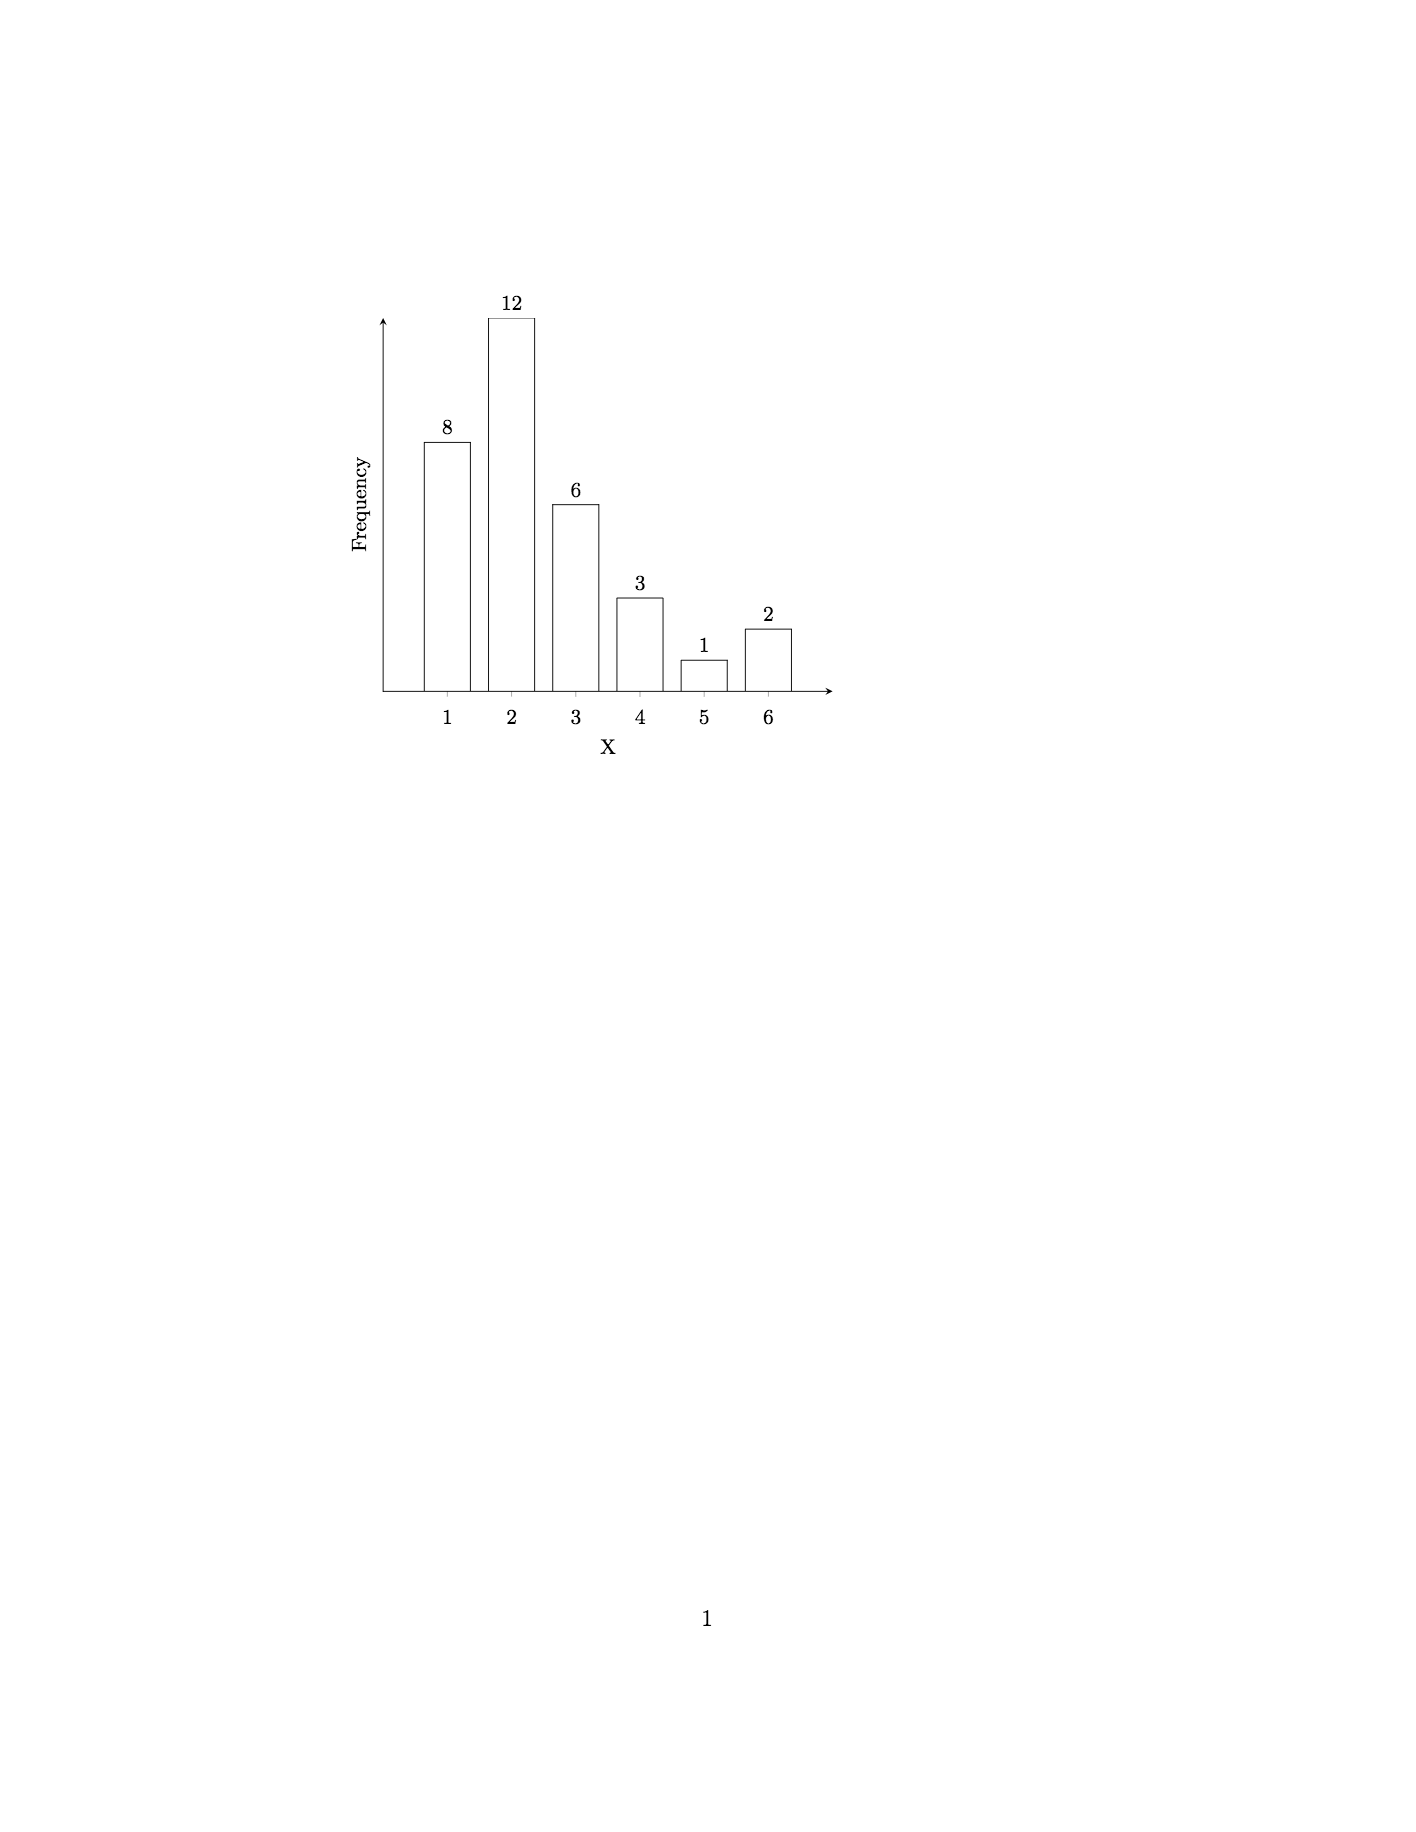
\includegraphics[width=1\linewidth]{images/frequencyhistogram.png}

		
		
%
\par
Experiment with creating your own histogram by inputting your data into the interactive cell below.
\begin{lstlisting}[style=sageinput]
#  This function is used to convert an input string into separate entries
def g(s): return str(s).replace(',',' ').replace('(',' ').replace(')',' ').split()

@interact
def _(freq = input_box("1,1,1,1,2,2,2,3,3,3,3,1,5",label="Enter data separated by commas")):
    freq = g(freq)
    freq = [int(k) for k in freq]
    m = min(freq)
    M = max(freq)
    bn = M-m+1
    histogram( freq, range=[m-1/2,M+1/2], bins = bn, align="mid", linewidth=2, edgecolor="blue", color="yellow").show()
\end{lstlisting}


		%
\par
Relative Frequency Histograms - In this case, area describes your data.  Notice in the interactive cell above that each bar is of width one. Therefore, frequency = area. In some instances where data may be grouped the total width of the interval may be different and so the height will need to be adjusted so that the total area of each bar corresponds to the relative frequency of that category.%
\par
Cummulative Histograms.  In these a running total is presented using all values from the given point and below.
\begin{lstlisting}[style=sageinput]
#  This function is used to convert an input string into separate entries
def g(s): return str(s).replace(',',' ').replace('(',' ').replace(')',' ').split()

@interact
def _(freq = input_box("1,1,1,1,2,2,2,3,3,3,3,1,5",label="Enter data separated by commas")):
    freq = g(freq)
    freq = [int(k) for k in freq]
    top = len(freq)
    m = min(freq)
    M = max(freq)
    bn = M-m+1
    histogram( freq, range=[m-1/2,M+1/2], cumulative = "true", bins = bn, align="mid", linewidth=2, edgecolor="blue", color="yellow").show(ymax=top)
\end{lstlisting}
		
		%
\par
Stem-and-Leaf Plot - Histogram with data. Using the state population data above, consider organizing the data but using a "two-pass sort" where you first roughly break data up into groups based upon ranges which relate to their first digit(s). In this case, let's break up into groups according to populations corresponding to 0-4 million, 5-9 million, 10-14 million, 15-19, million, 20-24 million, 25-29 million, 30-35 million, and 35-39 million. We can represent these classes by using the stems 0L, 0H, 1L, 1H, 2L, 2H, 3L, and 3H where the L and H represent the one's digits L in {0, 1, 2, 3, 4} and H in {5, 6, 7, 8, 9}.  Once we group the data into these smaller groups then we can write the remaining portion of the number horizontally as leaves (in this case with one decimal place for all values.) This gives a step-and-leaf plot. If we additionally sort the data in the leaves then this gives you an ordered stem-and-leaf plot. For the state population data, the ordered stem-and-leaf plot is given by
		

		
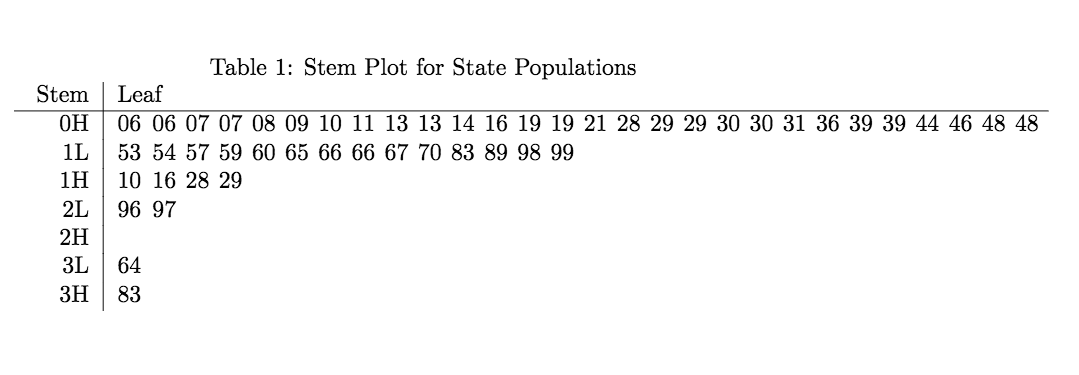
\includegraphics[width=1\linewidth]{images/stemandleaf.png}


Notice how it is easy to now see that most state populations are relatively small and that there are relatively few states with larger population. Also, notice that you can use this plot to relatively easily identify minimum, maximum, and other order statistics.		
		
		%
\par
Box and Whisker Diagram - visual order statistics. This graphical display identifies the "5-number-summary" associated with the minimum, quartiles, and the maximum. That is, \(y_1, Q_1, Q_2, Q_3, y_n\).  These values separate the data roughly into quarters. To distinguish these quarters connect \(y_1\) and \(Q_1\) with a straight line (a whisker) and do the same with \(Q_3\) and \(y_n\). Use a box to connect \(Q_1\) with \(Q_2\) and the same to connect \(Q_2\) with \(Q_3\). Then the boxed areas also identify the IQR.    
\begin{lstlisting}[style=sageinput]
from pylab import boxplot,savefig,close
@interact
def _(data = input_box([1,2,3,4,6,7,8,9,11,15,21],label="Enter Your Data:")):
    B = boxplot(data, notch=True, sym='x', vert=False)
    savefig("boxplot.png")
    close()
\end{lstlisting}

		%
\typeout{************************************************}
\typeout{Section 2.9 Exercises}
\typeout{************************************************}
\section[Exercises]{Exercises}\label{section-12}
Complete the online homework "Computational Measures".%
\par
Create a data set with about 10 elements. For your data set, compute each of the measures from this chapter and present your data using a frequency histogram.%
\par
Find a "real-world" data set (similar perhaps to the Census data presented above.) Compute each of the measures from this chapter. Interpret and present your conclusions in an electronic report which can include an excel spreadsheet.%
\typeout{************************************************}
\typeout{Chapter 3 Counting and Combinatorics}
\typeout{************************************************}
\chapter[Counting and Combinatorics]{Counting and Combinatorics}\label{Combinatorics}
\typeout{************************************************}
\typeout{Section 3.1 Introduction}
\typeout{************************************************}
\section[Introduction]{Introduction}\label{section-13}
Discussion on the usefulness of having ways to count the number
of elements in a set without having to explicitly listing all elements.%
\par
Consider counting the number of ways one can arrange Peter, Paul, and Mary with the order important.  Listing the possibilities:
\leavevmode%
\begin{itemize}[label=\textbullet]
\item{}Peter, Paul, Mary%
\item{}Peter, Mary, Paul%
\item{}Paul, Peter, Mary%
\item{}Paul, Mary, Peter%
\item{}Mary, Peter, Paul%
\item{}Mary, Paul, Peter%
\end{itemize}

So, it is easy to see that these are all of the possible outcomes and that the total number of such outcomes is 6. What happens however if we add Simone to the list?
\leavevmode%
\begin{itemize}[label=\textbullet]
\item{}Simone, Peter, Paul, Mary%
\item{}Simone, Peter, Mary, Paul%
\item{}Simone, Paul, Peter, Mary%
\item{}Simone, Paul, Mary, Peter%
\item{}Simone, Mary, Peter, Paul%
\item{}Simone, Mary, Paul, Peter%
\item{}Peter, Simone, Paul, Mary%
\item{}Peter, Simone, Mary, Paul%
\item{}Paul, Simone, Peter, Mary%
\item{}Paul, Simone, Mary, Peter%
\item{}Mary, Simone, Peter, Paul%
\item{}Mary, Simone, Paul, Peter%
\item{}Peter, Paul, Simone, Mary%
\item{}Peter, Mary, Simone, Paul%
\item{}Paul, Peter, Simone, Mary%
\item{}Paul, Mary, Simone, Peter%
\item{}Mary, Peter, Simone, Paul%
\item{}Mary, Paul, Simone, Peter%
\item{}Peter, Paul, Mary, Simone%
\item{}Peter, Mary, Paul, Simone%
\item{}Paul, Peter, Mary, Simone%
\item{}Paul, Mary, Peter, Simone%
\item{}Mary, Peter, Paul, Simone%
\item{}Mary, Paul, Peter, Simone%
\end{itemize}

Notice how the list quickly grows when just adding one more choice. This illustrates how keeping track of the number of items in a set can quickly get impossible to keep up with and to count unless we can approach this problem using a more mathematical approach.
%
\begin{definition}[Cardinality]\label{definition-17}
Given a set of elements A, the number of elements in the 
		set is known as the sets cardinality and is denoted |A|. If the set has 
		an infinite number of elements then we set |A| = \(\infty\).
		\end{definition}
\par
In order to "count without counting" we establish the following 
	foundational principle.%
\begin{theorem}[Multiplication Principle]\label{theorem-9}
Given two successive events A and B, the number of ways 
		to perform A and then B is |A||B|.
		\end{theorem}
\begin{proof}\hypertarget{proof-6}{}
If either of the events has infinite cardinality, then it is 
			clear
			that the number of ways to perform A and then B will also be 
			infinite. So, assume that both |A| and |B| are finite.
			In order to count the successive events, enumerate the elements in
			each set
			\begin{gather*}
A = \left \{ a_1, a_2, a_3, ... , a_{|A|} \right \}\\
B = \left \{  b_1, b_2, b_3, ... , b_{|B|} \right \}
\end{gather*}
			and consider the function f(k,j) = (k-1)|B| + j. This function is 
			one-to-one and onto from the set 
			\begin{gather*}
\left \{ (k,j): 1 \le k \le |A|, 1 \le j \le |B| \right \} 
\end{gather*} 
			onto 
			\begin{gather*}
\left \{ s : 1 \le s \le |A| |B| \right \}.
\end{gather*} 
			Since this
			second set has |A| |B| elements then the conclusion follows. 
			coordinates.%
\end{proof}
\begin{definition}[Factorial]\label{definition-18}
For any natural number n, 
		\begin{gather*}
n! = n(n-1)(n-2) ... 3 \cdot 2 \cdot 1
\end{gather*}
		%
\end{definition}
\begin{example}[iPad security code]\label{example-8}
Consider your ipad's security. To unlock the screen you need to enter your four digit pass code. How easy is it to guess this pass code?%
\par
Using the standard 10 digit keypad, we first have two questions to consider?
		\leavevmode%
\begin{enumerate}
\item\hypertarget{li-74}{}Does the order in which the digits are entered matter?%
\item\hypertarget{li-75}{}Can you reuse a digit more than once?%
\end{enumerate}

		For the ipad, the order does matter and you cannot reuse digits. In this case, the number of possible codes can be determined by considering each digit as a separate event with four such events in succession providing the right code. By successively applying the multiplication principle, you find that the number of possible codes is the number of remaining available digits at each step.  Namely, \(10 \times 9 \times 8 \times 7 = 5040.\)
		%
\par

		Note that if you were allowed to reuse the digits then the number of possible outcomes would be more since all 10 digits would be available for each event.  Namely, \(10 \times 10 \times 10 \times 10 = 10000.\)
		%
\end{example}
\begin{example}[iPad security code with greasy fingers]\label{example-9}
Reconsider your ipad's security. In this case, you like to eat
		chocolate bars and have greasy fingers. When you type in your passcode
		your fingers leave a residue over the four numbers pressed. If someone
		now tries to guess your passcode, how many possible attempts are necessary?%
\par
Since there are only four numbers to pick from with order important, the number of possible passcodes remaining is \(4 \times 3 \times 2 \times 1 = 24\)%
\end{example}
\begin{example}[National Treasure]\label{example-10}
In the 2004 movie "National Treasure" Ben and Riley are attempting 
		to guess Abagail's password to enter the room with the Declaration. 
		They are able
		to determine the passphrase to get into the vault room by doing a scan
		that detects the buttons pushed (not due to chocolate but just due to 
		the natural oils on fingers). They notice that the buttons pushed 
		include the characters AEFGLORVY.%
\par
Assuming these characters are used only once each, how many possible
		passphrases are possible?%
\par

		In this case, the order of the characters matters but all of the 
		characters are distinct. Since we have 9 characters provided, the we can
		consider each character as an event with the first event as a choice
		from the 9, the second event as a choice from the remaining 8, etc. This
		gives \(9 \times 8 \ times ... \times 1 = 362880\) possible 
		passphrases.
		%
\par
Assuming that some of the characters could be used more than once, 
		how many passphrases need to be considered if the total length
		of passphrase can be at most 12 characters?%
\par
Notice, in this case you don't know which characters might be reused and so the number of possible outcomes will be much larger. What is the answer?%
\par
You can break this problem down into distinct cases:
		\leavevmode%
\begin{itemize}[label=\textbullet]
\item{}Using 9 characters
			This is the answer computed above.%
\item{}Using 10 characters
			In this case, 1 character can be used twice. To determine the number of possibilities, let's first pick which character can be doubled. There are 9 options for picking that character.  Next, if we consider the two instances of that letter as distinct values then we can just count the number of ways to arrange unique 10 characters which is 10! However, swapping the two characters (which are actually identical) would not give a new passphrase. Since these are counted twice, let's divide these out to give 10!/2.%
\item{}Using 11 characters
				In this situation we have two unique options:
				%
\begin{itemize}[label=$\circ$]
\item{}One character is used three times and the others just once.
					Continuing as in the previous case, 11!/3!.%
Two characters are used twice and the others just once.\end{itemize}

				%
\item{}Using 12 characters%
%
\begin{enumerate}
\item\hypertarget{li-82}{}One letter from the nine is used four times and all the others are used once.%
\item\hypertarget{li-83}{}One letter is used three times, another letter is used two times, and the others are used once.%
\item\hypertarget{li-84}{}Three letters are used twice and the others are used once.%
\end{enumerate}
\end{itemize}

			%
\par
With this large collection of possible outcomes, how are the movie
		characters able to determine the correct "VALLEYFORGE" passphrase?%
\end{example}
\typeout{************************************************}
\typeout{Section 3.2 Permutations}
\typeout{************************************************}
\section[Permutations]{Permutations}\label{section-14}
When counting various outcomes the order of things sometimes matters. When the order of a set of elements changes we call the second a permutation (or an arrangement) of the first.%
\begin{theorem}[Permutations of n objects]\label{theorem-10}
The number of ways to arrange n distinct items is n!\end{theorem}
\begin{proof}\hypertarget{proof-7}{}
Notice that if n=1, then there is only 1 item to arrange and 
			that there is only one possible arrangment.%
\par

			By induction, assume that any set with n elements has n! arrangments 
			and assume that 
			\begin{gather*}
|A| = \left \{ a_1, a_2, ... , a_n, a_{n+1} \right \}.
\end{gather*}
			Notice that there are n+1 ways to choose 1 element from A and that in doing so leaves a set with n elements. Combining the induction hypothesis with the multiplication principle this gives (n+1)n! = (n+1)! possible outcomes.
			%
\end{proof}
\begin{theorem}[Permutations of n objects selecting r]\label{theorem-11}

			The number of ways to arrange r items from a set of n distinct items 
			is \( P_r^n = \frac{n!}{(n-r)!} \)
			%
\end{theorem}
\begin{proof}\hypertarget{proof-8}{}

			Apply the multiplication principle r times noting that there are 
			n choices for the first selection, n-1 choices for the second
			selection, and with n-r+1 choices for the rth selection. This gives
			\begin{align*}
P_r^n & = n(n-1) ... (n-r+1)\\
& = n(n-1) ... (n-r+1)\frac{(n-r)!}{(n-r)!}\\
& = \frac{n(n-1) ... (n-r+1)(n-r)!}{(n-r)!}\\
& = \frac{n!}{(n-r)!}
\end{align*}
			%
\end{proof}
\begin{theorem}[Permutations when Not all items are distinguishable and without replacement: (Multinomial Coefficients)]\label{theorem-12}

If n items belong to s categories, n1 in first, n2 in second, ... , ns in the last, the number of ways to pick all is
!	
	\end{theorem}
\typeout{************************************************}
\typeout{Section 3.3 Combinations}
\typeout{************************************************}
\section[Combinations]{Combinations}\label{section-15}
When counting various outcomes sometimes the order of things does not matter.
In this case we count each different set of outcomes a combination. %
\begin{theorem}[Combinations of n distinct objects selecting r without replacement]\label{theorem-13}

			The number of ways to arrange r items from a set of n distinct items 
			is \( C_r^n = \frac{n!}{r!(n-r)!} \)
			%
\end{theorem}
\begin{proof}\hypertarget{proof-9}{}

			Consider creating a permutation of r objects from a set of size n
			by first picking an unordered subset of size r and then counting 
			the number of ways to order that subset. Using our notation and the
			multiplication principle,
			\begin{gather*}
P_r^n = C_r^n \cdot r!
\end{gather*}
			Solving give the result.
			%
\end{proof}
\begin{theorem}[Combinations of n distinct objects selecting r with replacement]\label{theorem-14}

			The number of ways to arrange r items from a set of n distinct items 
			is \( C_r^{n+r-1} = \frac{n+r-1!}{r!(n-1)!} \)
			%
\end{theorem}
\begin{proof}\hypertarget{proof-10}{}

			blah
			%
\end{proof}
\begin{example}[]\label{example-11}
Revisiting your ipad's security, what happens if the order in which the digits are entered does not matter? If so, then you would be picking a combination of 4 digits without replacement from a group of 10 digits. Namely, 
		\begin{align*}
\frac{10!}{4!6!} & = \frac{10 \times 9 \times 8 \times 7 \times 6!}{4 \times 3 \times 2 \times 1 \times 6!}\\
& = \frac{10 \times 9 \times 8 \times 7}{4 \times 3 \times 2 \times 1}\\
& = \frac{5040}{24}\\
& = 210.
\end{align*}
		Notice that the total number of options is much smaller when order does not matter.
		%
\par

		Note that if you were allowed to reuse the digits then the number of possible outcomes would be
		\begin{align*}
\frac{13!}{3!10!} & = \frac{13 \times 12 \times 11}{3 \times 2 \times 1} \\
 & = 286
\end{align*}
		which once again is more since numbers are allowed to repeat.
		%
\end{example}
\begin{definition}[Binomial Coefficients]\label{definition-19}

		The value \(C_r^n\) is known as the binomial coefficient. It is
		denoted by \({n \choose r}\) and is read "n choose k".
		%
\end{definition}
\begin{theorem}[Combinations when distinguishable and with replacement]\label{theorem-15}

	= Number of ways to get unordered samples of size r from n objects. 
	\end{theorem}
\par
Lots of interesting facts about the binomial coefficients.%
\typeout{************************************************}
\typeout{Section 3.4 Exercises}
\typeout{************************************************}
\section[Exercises]{Exercises}\label{section-16}
Complete the online homework "Counting".%
\par
Completely determine the number of possible passphrases for the National Treasure example started above. Present your answer in a report form.%
\typeout{************************************************}
\typeout{Chapter 4 Probability and Probability Functions}
\typeout{************************************************}
\chapter[Probability and Probability Functions]{Probability and Probability Functions}\label{ProbabilityGeneralities}
\typeout{************************************************}
\typeout{Introduction  }
\typeout{************************************************}
This chapter is a definitions of probability, consequences, and probability functions.%
\typeout{************************************************}
\typeout{Section 4.1 Relative Frequency}
\typeout{************************************************}
\section[Relative Frequency]{Relative Frequency}\label{RelativeFrequency}
Mathematics generally focuses on providing precise answers with absolute certainty. For example, solving an equation generates specific (and non-varying) solutions. Statistics on the other hand deals with providing precise answers to questions when there is uncertainty. It might seem impossible to provide such precise answers but the focus of this text is to show how that can be done so long as the questions are properly posed and the answers properly interpreted.%
\par
People often make claims about being the biggest, best, most often recommended, etc. One sometimes even believes these claims. In this class, we will attempt to determine if such claims are reasonable by first introducing probability from a semi rigorous mathematical viewpoint using concepts developed in Calculus. We will use this framework to carefully discuss making such statistical inferences as above and in general to obtain accurate knowledge even when the known data is not complete. %
\par
When attempting to precisely measure this uncertainty a few experiments are in order. When doing statistical experiments, a few terms and corresponding notation might be useful:%
\leavevmode%
\begin{itemize}[label=\textbullet]
\item{}S = Universal Set or Sample Space Experiment or Outcome Space. 
		This is the collection of all possible outcomes.%
\item{}Random Experiment. A random experiment is a repeatable activity which has more than one
		possible outcome all of which can be specified in advance but can not be known in advance with certainty.%
\item{}Trial. Performing a Random Experiment one time and measuring the result.%
\item{}A = Event. A collection of outcomes.  Generally denoted by an upper case letter such as A, B, C, etc.%
\item{}Success/Failure. When recording the result of a trial, a success for event A occurs when the outcome
		lies in A. If not, then the trial was a failure. There is no qualitative meaning to this term.%
\item{}Mutually Exclusive Events. Two events which share no common outcomes. Also known as disjoint events.%
\item{}|A| = Frequency. In a sequence of n events, the frequency is the number of trials which resulted in 
		a success for event A.%
\item{}|A| / n = Relative Frequency. A proportion of successes to total number of trials.%
\item{}Histogram. A bar chart representation of data where area corresponds to the value being described.%
\end{itemize}
\par
To investigate these terms and to motivate our discussion of probability, consider flipping coins using the interactive cell below. Notice in this case, the sample space S = {Heads, Tails} and the random experiment consists of flipping a fair coin one time. Each trial results in either a Head or a Tail. Since we are measuring both Heads and Tails then we will not worry about which is a success or failure. Further, on each flip the outcomes of Heads or Tails are mutually exclusive events. We count the frequencies and compute the relative frequencies for a varying number of trials selected by you as you move the slider bar. Results are displayed using a histogram.%
\par

	Question 1: What do you notice as the number of flips increases?
	%
\par

	Question 2: Why do you rarely (if even) get exactly the same number of Heads and Tails? Would you not "expect"
	that to happen?
	%
\begin{lstlisting}[style=sageinput]
coin = ["Heads", "Tails"]
@interact
def _(num_rolls = slider([5..5000],label="Number of Flips")):
	rolls = [choice(coin) for roll in range(num_rolls)]
	show(rolls)   
	freq = [0,0]
	for outcome in rolls:
		if (outcome=='Tails'):
			freq[0] = freq[0]+1
		else:
			freq[1] = freq[1]+1
	print("\nThe frequency of tails = "+ str(freq[0]))+" and heads = "+ str(freq[1])+"."
	rel = [freq[0]/num_rolls,freq[1]/num_rolls]
	print("\nThe relative frequencies for Tails and Heads:"+str(rel))
	show(bar_chart(freq,axes=False,ymin=0))     #  A histogram of the results
\end{lstlisting}
\par
Notice that as the number of flips increases, the relative frequency of Heads (and Tails)
	stabilized around 0.5. This makes sense intuitively since there are two options for each 
	individual flip and 1/2 of those options are Heads while the other 1/2 is Tails.%
\par

	Let's try again
	by doing a random experiment consisting of rolling a single die one time. Note that the sample space 
	in this case will be the outcomes S = {1, 2, 3, 4, 5, 6}.
	%
\par

	Question 1: What do you notice as the number of rolls increases?
	%
\par

	Question 2: What do you expect for the relative frequencies and why are they not all exactly the same?
	%
\begin{lstlisting}[style=sageinput]
@interact
def _(num_rolls = slider([20..5000],label='Number of rolls'),Number_of_Sides = [4,6,8,12,20]):
	die = list((1..Number_of_Sides))
	rolls = [choice(die) for roll in range(num_rolls)]
	show(rolls)   

	freq = [rolls.count(outcome) for outcome in set(die)]  # count the numbers for each outcome
	print 'The frequencies of each outcome is '+str(freq)

	print 'The relative frequencies of each outcome:'
	rel_freq = [freq[outcome-1]/num_rolls for outcome in set(die)]  # make frequencies relative
	print rel_freq
	fs = []
	for f in rel_freq:
		fs.append(f.n(digits=4))
	print fs
	show(bar_chart(freq,axes=False,ymin=0))
\end{lstlisting}
\par
Notice in this instance that there are a larger number of options (for example 6 on a regular
	die) but once again the relative frequencies of each  outcome was close to 1/n (i.e. 1/6 for the regular die)
	as the number of rolls increased.%
\par
In general, this suggests a rule: if there are n outcomes and each one has the same
	chance of occurring on a given trial then on average on a large number of trials the relative
	frequency of that outcome is 1/n.
	In general, if a number of outcomes are "equally likely" then this is a good model for measuring
	the proportion of outcomes that would be expected to have any given outcome. However, it is not
	always true that outcomes are equally likely. Consider rolling two die and measuring their sum:%
\begin{lstlisting}[style=sageinput]
@interact
def _(num_rolls = slider([20..5000],label='Number of rolls'),num_sides = slider(4,20,1,6,label='Number of sides')):
    die = list((1..num_sides))
    dice = list((2..num_sides*2))
    rolls = [(choice(die),choice(die)) for roll in range(num_rolls)]
    sums = [sum(rolls[roll]) for roll in range(num_rolls)]
    show(rolls)   

    freq = [sums.count(outcome) for outcome in set(dice)]  # count the numbers for each outcome
    print 'The frequencies of each outcome is '+str(freq)
    
    print 'The relative frequencies of each outcome:'
    rel_freq = [freq[outcome-2]/num_rolls for outcome in set(dice)]  # make frequencies relative
    print rel_freq        
    show(bar_chart(freq,axes=False,ymin=0))     #  A histogram of the results
    print "Relative Frequence of ",dice[0]," is about ",rel_freq[0].n(digits=4)
    print "Relative Frequence of ",dice[num_sides-1]," is about ",rel_freq[num_sides-1].n(digits=4)
\end{lstlisting}
\par
Notice, not only are the answers not the same but they are not even close. To understand why this 
	is different from the examples before, consider the possible outcomes from each pair of die. Since we
	are measuring the sum of the dice then (for a pair of standard 6-sided dice) the possible sums are from 
	2 to 12. However, there is only one way to get a 2--namely from a (1,1) pair--while there are 6 ways to get
	a 7--namely from the pairs (1,6), (2,5), (3,4), (4,3), (5,2), and (6,1). So it might make some sense
	that the likelihood of getting a 7 is 6 times larger than that of getting a 2. Check to see if that
	is the case with your experiment above.%
\typeout{************************************************}
\typeout{Section 4.2 Definition of Probability}
\typeout{************************************************}
\section[Definition of Probability]{Definition of Probability}\label{section-18}
\typeout{************************************************}
\typeout{Subsection 4.2.1 Motivating the Definition}
\typeout{************************************************}
\subsection[Motivating the Definition]{Motivating the Definition}\label{ProbabilityDefns}
Using the ideas from our examples above, let's consider how we might formally define a way
	to measure the expectation from similar experiments.  Before doing so, we need a little notation:%
\begin{definition}[]\label{definition-20}
The Cardinality of the set A is the number of elements in A. This will be denoted |A| (similar
		to the idea of frequency of an outcome noted earlier.) If a set has
		a infinite number of elements, then we will say it's cardinality is also infinite and 
		write |A| = \(\infty\)\end{definition}
\begin{definition}[Pairwise Disjoint Sets]\label{definition-21}
\( \{ A_1, A_2, ... , A_n \}\) are pairwise disjoint provided \(A_k \cap A_j = \emptyset\) so long as \(k \ne j\).
		\end{definition}
\par

	To model the behavior above, consider how we might create a definition for our expectation
	of a given outcome by following the ideas uncovered above. To do so, first consider a desired collection
	of outcomes A. If each outcome in A is equally likely then we might follow the concept behind relative 
	frequency and consider a measure of expectation be |A|/|S|. Indeed, on a standard 
	6-sided die, the expectation of the outcome A={2} from the collection S = {1,2,3,4,5,6} should be
	|A|/|S| = 1/6.%
\par
From the example where we take the sum of two die, the outcome A={4,5} from the
	collection S = {2,3,4,...,12} would be%
\begin{gather*}
|A| = | {(1,3),(2,2),(3,1),(1,4),(2,3),(3,2),(4,1)}| = 7\\
|S| = | {(1,1),...,(1,6),(2,1),...,(2,6),...,(6,1),...,(6,6)}| = 36
\end{gather*}\par
and so the expected relative frequency would be |A|/|S| = 7/36. Compare this theoretical value
	with the sum of the two outcomes from your experiment above.%
\par
We are ready to now formally give a name to the theoretical measure of expectation for
	outcomes from an experiment. Taking our cue from the ideas related to equally likely outcomes, we 
	make our definition have the following basic properties:%
\leavevmode%
\begin{enumerate}
\item\hypertarget{li-94}{}Relative frequency cannot be negative, since cardinality cannot be negative%
\item\hypertarget{li-95}{}Relative frequencies for disjoint events should sum to one%
\item\hypertarget{li-96}{}Relative frequencies for collections of disjoint outcomes should equal the sum of the
	individual relative frequencies%
\end{enumerate}
\typeout{************************************************}
\typeout{Subsection 4.2.2 Probability}
\typeout{************************************************}
\subsection[Probability]{Probability}\label{subsection-9}
Based upon these we give the following:%
\begin{definition}[]\label{DefnProb}
The probability P(A) of a given outcome A is a set function which satisfies:
		\leavevmode%
\begin{enumerate}
\item\hypertarget{li-97}{}(Nonnegativity) P(A) \(\ge 0\)%
\item\hypertarget{li-98}{}(Totality) P(S) = 1%
\item\hypertarget{li-99}{}(Subadditivity) If A \(\cap\) B = \(\emptyset\), then P(A \(\cup\) B) = P(A) + P(B).  
			In general, if {\(A_k\)} are pairwise disjoint then \(P( \cup_k A_k) = \sum_k P(A_k)\).%
\end{enumerate}
\end{definition}
\typeout{************************************************}
\typeout{Subsection 4.2.3 Basic Probability Theorems}
\typeout{************************************************}
\subsection[Basic Probability Theorems]{Basic Probability Theorems}\label{BasicProbabilityTheorems}
Based upon this definition we can immediately establish a number of results.%
\begin{theorem}[Probability of Complements]\label{ProbabilityComplemnts}
 For any event A, \(P(A) + P(A^c) = 1\)\end{theorem}
\begin{proof}\hypertarget{proof-11}{}
Let A be any event and note that \(A \cap A^c = \emptyset\).  But \(A \cup A^c = S\).
			So, by subadditivity \(1 = P(S) = P(A \cup A^c) = P(A) + P(A^c)\) as desired.%
\end{proof}
\begin{theorem}[]\label{ProbabilityEmptySet}
\(P(\emptyset) = 0\)\end{theorem}
\begin{proof}\hypertarget{proof-12}{}
Note that \(\emptyset^c = S\). So, by the theorem above, 
			\(1 = P(S) + P(\emptyset) \Rightarrow 1 = 1 + P(\emptyset)\).
			Cancelling the 1 on both sides gives \(P(\emptyset) = 0\). %
\end{proof}
\begin{theorem}[]\label{ProbabilityContainment}
For events A and B with \( A \subset B, P(A) \le P(B)\).
		\end{theorem}
\begin{proof}\hypertarget{proof-13}{}
Assume sets A and B satisfy \( A \subset B\). Then, notice that
			\(A \cap (B-A) = \emptyset\) and  \(B = A \cup (B-A)\). Therefore, by 
			subadditivity and nonnegativity%
\begin{gather*}
0 \le P(B-A)\\
P(A) \le P(A) + P(B-A) \\
P(A) \le P(B)
\end{gather*}\end{proof}
\begin{theorem}[]\label{ProbabilityLessThanOne}
For any event A, \(P(A) \le 1\)\end{theorem}
\begin{proof}\hypertarget{proof-14}{}
Notice \(A \subset S\). By the theorem above \( P(A) \le P(S) = 1\)%
\end{proof}
\begin{theorem}[]\label{ProbabilityTwoUnions}
For any sets A and B, \(P(A \cup B) = P(A) + P(B) - P(A \cap B)\)\end{theorem}
\begin{proof}\hypertarget{proof-15}{}
Notice that we can write \(A \cup B\) as the disjoint union%
\begin{gather*}
A \cup B = (A-B) \cup (A \cap B) \cup (B-A).
\end{gather*}\par
We can also write disjointly%
\begin{gather*}
A = (A-B) \cup (A \cap B)\\
B = (A \cap B) \cup (B-A)
\end{gather*}\par
Hence, %
\begin{align*}
P(A) & + P(B) - P(A \cap B) \\
& = [P(A-B) + P(A \cap B)] + [P(A \cap B) + P(B-A)] - P(A \cap B)\\
& = P(A-B) + P(A \cap B) + P(B-A)\\
& = P(A \cup B)
\end{align*}\end{proof}
\par
This result can be extended to more that two sets using a property known as inclusion-exclusion. The
	following two theorems illustrate this property and are presented without proof.
	%
\begin{corollary}[]\label{ProbabilityThreeUnions}

			For any sets A, B and C, 
			\begin{align*}
P(A \cup B \cup C) & = P(A) + P(B) + P(C)\\
& - P(A \cap B) - P(A \cap C) - P(B \cap C) \\
& + P(A \cap B \cap C)
\end{align*}\end{corollary}
\begin{corollary}[]\label{ProbabilityFourUnions}

			For any sets A, B, C and D, 
			\begin{align*}
P(A \cup B \cup C \cup D) & = P(A) + P(B) + P(C) + P(D)\\
& - P(A \cap B) - P(A \cap C) - P(A \cap D)  - P(B \cap C) - P(B \cap D) - P(C \cap D)\\
& + P(A \cap B \cap C) + P(A \cap B \cap D) + P(A \cap C \cap D) + P(B \cap C \cap D)\\
& - P(A \cap B \cap C \cap D)
\end{align*}\end{corollary}
\typeout{************************************************}
\typeout{Section 4.3 Conditional Probability}
\typeout{************************************************}
\section[Conditional Probability]{Conditional Probability}\label{section-19}
\begin{example}[Changing Sample Space - Balls]\label{example-12}
Consider a box with three balls: one Red, one White, and one Blue.  Using an equally likely assumption, the probability of randomly pulling out a Red ball should be 1/3.  That is P(Red) = 1/3.  However, suppose that for a first trial you pull out the White ball and set it aside. Attempting to pull out another ball leaves you with only two options and so the probability of randomly pulling out a Red ball is 1/2. Notice that the probability changed for the second trial dependent on the outcome of the first trial.%
\end{example}
\begin{example}[Changing Sample Space - Cards]\label{example-13}
Consider a deck of 52 standard playing cards and a success occurs when a Heart is selected from the deck. 
	When extracting one card randomly, the probability	of that card being a Heart is then P(Heart) = 13/52. Now, assume that one card has already been extracted and setaside.  Now, prepare to extract another. If the first card drawn was a Heart, then there are only 12 Hearts left for the second draw. However, if the first card drawn was not a Heart, then there are 13 Hearts available for the second draw. To compute this probability correctly, one need to formulate the question so that subadditivity can  be utilized.%
\par

	To do this, consider 
	P(Heart on 2nd draw) 
	= P( [Heart on 1st draw \(\cap\) Heart on 2nd draw] \(\cup\) [Not Heart on 1st draw \(\cap\) Heart on 2nd draw] )
	= P(Heart on 1st draw \(\cap\) Heart on 2nd draw ) + P(Not Heart on 1st draw \(\cap\) Heart on 2nd draw )
	= | Heart on 1st draw \(\cap\) Heart on 2nd draw | / | Number of ways to get two cards |
	+ | Not Heart on 1st draw \(\cap\) Heart on 2nd draw / | Number of ways to get two cards |
	= (13 12) / (52 51) + (39 13) / (52 51) = 12 / (4 51) + (3 13) / ( 4 51) =  

	%
\end{example}
\begin{definition}[Conditional Probability]\label{definition-23}
P(B | A) = P(A \(\cap\) B) / P(A), provided P(A)\(\gt 0\).\end{definition}
\begin{theorem}[]\label{theorem-21}
Conditional Probability satisfies all of the requirements of regular probability.\end{theorem}
\begin{proof}\hypertarget{proof-16}{}

		By definition, for any event probability must be nonnegative. Therefore
		\(P(A \cap B) \ge 0\).  Therefore, P(B | A) \(\ge 0\).
		%
\par

		Further, P (S | A) = P(A \(\cap\) S)/P(A) = P(A)/P(A) = 1.
		%
\end{proof}
\begin{theorem}[Multiplication Rule]\label{theorem-22}
\begin{equation*}P(A \cap B) = P(A) P(B | A) = P(B) P(A | B)\end{equation*}\end{theorem}
\begin{proof}\hypertarget{proof-17}{}

		Unravel the definition of conditional probably by taking the denominator to the other side. Also note that you can write \(A \cap B = B \cap A\).
		%
\end{proof}
\typeout{************************************************}
\typeout{Section 4.4 Bayes Theorem}
\typeout{************************************************}
\section[Bayes Theorem]{Bayes Theorem}\label{section-20}
\begin{theorem}[Bayes Theorem]\label{theorem-23}
Let \(S = \{ S_1, S_2, ... , S_m \}\) where the \(S_k\) are pairwise disjoint and \(S_1 \cup S_2 \cup ... \cup S_m = S\) (i.e. a partition of the space S).  Then for any \(A \subset S\)\begin{gather*}
P(S_j | A) = \frac{P(S_j)P(A | S_j)}{\sum_{k=1}^m P(S_k)P(A | S_k)}.
\end{gather*}
		The conditional probability \(P(S_j | A)\) is called the posterior probability of \(S_k\).
		\end{theorem}
\begin{proof}\hypertarget{proof-18}{}

		Notice, by the definition of conditional probability and the multiplication rule
		\begin{equation*}P(S_j | A) = \frac{P(S_j \cap A)}{P(A)} = \frac{P(S_j)P( A | S_j)}{P(A)}.\end{equation*}
		But using the disjointness of the partition 
		\begin{align*}
P(A) & = P( (A \cap S_1) \cup (A \cup S_2) \cup ... \cup (A \cup S_m) )\\
    & = P(A \cap S_1) + P(A \cup S_2) + ... + P(A \cup S_m)\\
    & = P(S_1 \cap A) + P(S_2 \cup A) + ... + P(S_m \cup A)\\
    & = P(S_1) P(A | S_1) + P(S_2)P(A | S_2) + ... + P(S_m)P(A | S_m)\\
    & = \sum_{k=1}^m P(S_k)P(A | S_k)
\end{align*}
		Put these two expansions together to obtain the desired result.
		%
\end{proof}
\begin{lstlisting}[style=sageinput]
#  This function is used to convert an input string into separate entries
def g(s): return str(s).replace(',',' ').replace('(',' ').replace(')',' ').split()

@interact
def _(Partition_Probabilities=input_box('0.35,0.25,0.40',label="$P(B_1),P(B_2),...$"),
        Conditional_Probabilities=input_box('0.02,0.01,0.03',label='$P(A|B_1),P(A|B_2),...$'),
        print_numbers=checkbox(True,label='Numerical Results on Graphs?'),
        auto_update=False):
            
    Partition_Probabilities = g(Partition_Probabilities)
    Conditional_Probabilities = g(Conditional_Probabilities)
    n = len(Partition_Probabilities)
    n0 = len(Conditional_Probabilities)
    
    # below needs to be n not equal to n0 but mathbook xml will not let me get the other
    if (n > n0):
        pretty_print("You must have the same number of partition probabilities and conditional probabilities.")
        
    else:                               # input data streams now are the same size!
        colors = rainbow(n)
        accum = float(0)                # to test whether partition probs sum to one
        ends = [0]                      # where the graphed partition sectors change in pie chart 
        mid = []                        # middle of each pie chart sector used for placement of text
        p_Bk_given_A = []               # P( B_k | A )
        pA = 0                          # P(A)
        PP=[]                           # array to hold the numerical Partition Probabilities 
        CP=[]                           # array to hold the numerical Conditional Probabilities     
        for k in range(n):
            PP.append(float(Partition_Probabilities[k]))
            CP.append(float(Conditional_Probabilities[k]))    
            p_Bk_given_A.append(PP[k]*CP[k] )
            pA += p_Bk_given_A[k]
            accum = accum + PP[k]
            ends.append(accum)
            mid.append((ends[k]+accum)/2)
#
#  Marching along from 0 to 1, saving angles for each partition sector boundary.
#  Later, we will multiple these by 2*pi to get actual sector boundary angles.
#
        if abs(accum-float(1))>0.0000001:     #  Due to roundoff issues, this should be close enough.                     
            pretty_print("Sum of probabilities should equal 1.")
        
        else:                           # probability data is sensible
 
#        
#  Draw the Venn diagram by drawing sectors from the angles determined above
#  First, create a circle of radius 1 to illustrate the the sample space S
#  Then draw each sector with varying colors and print out their names on the edge
#
            G = circle((0,0), 1, rgbcolor='black',fill=False, alpha=0.4,aspect_ratio=True,axes=False,thickness=5)
            for k in range(n):
                G += disk((0,0), 1, (ends[k]*2*pi, ends[k+1]*2*pi), color=colors[mod(k,10)],alpha = 0.2)
                G += text('$B_'+str(k+1)+'$',(1.1*cos(mid[k]*2*pi), 1.1*sin(mid[k]*2*pi)), rgbcolor='black')
                
            G += circle((0,0), 0.6, facecolor='yellow', fill = True, alpha = 0.1, thickness=5,edgecolor='black') 
    
#  Print the probabilities corresponding to each particular region as a list and on the graphs
            if print_numbers:               

                html("$P(A) = %s$"%(str(pA),))
                for k in range(n):
                    html("$P(B_{%s} | A)$"%(str(k+1))+"$ = %s$"%str(p_Bk_given_A[k]/pA))
                                        
                    G += text(str(p_Bk_given_A[k]),(0.4*cos(mid[k]*2*pi), 0.4*sin(mid[k]*2*pi)), rgbcolor='black')
                    G += text(str(PP[k] - p_Bk_given_A[k]),(0.8*cos(mid[k]*2*pi), 0.8*sin(mid[k]*2*pi)), rgbcolor='black')
        
#  This is essentially a repeat of some of the above code but focused only on creating the smaller inner circle dealing
#  with the set A so that the sectors now correspond in area to the Bayes Theorem probabilities


            accum = float(0)                        
            ends = [0]                     # where the graphed partition sectors change in pie chart 
            mid = []                       # middle of each pie chart sector used for placement of text
            for k in range(n): 
                accum += float(p_Bk_given_A[k]/pA) 
                ends.append(accum)
                mid.append((ends[k]+accum)/2)
            H = circle((0,0), 1, rgbcolor='black',fill=False, alpha=0,aspect_ratio=True,axes=False,thickness=0)
            H += circle((0,0), 0.6, facecolor='yellow',fill=True, alpha=0.1,aspect_ratio=True,axes=False,thickness=5,edgecolor='black')
            
            for k in range(n):
                H += disk((0,0), 0.6, (ends[k]*2*pi, ends[k+1]*2*pi), color=colors[mod(k,10)],alpha = 0.2)
                H += text('$B_'+str(k+1)+'|A$',(0.7*cos(mid[k]*2*pi), 0.7*sin(mid[k]*2*pi)), rgbcolor='black')
                    
        #  Now, print out the bayesian probabilities using the smaller set A only
    
            if print_numbers:
                for k in range(n):
                    H += text(str( N(p_Bk_given_A[k]/pA,digits=4) ),(0.4*cos(mid[k]*2*pi), 0.4*sin(mid[k]*2*pi)), rgbcolor='black')
                    
            G.show(title='Venn diagram of partition with A in middle')
            print
            H.show(title='Venn diagram presuming A has occured')
\end{lstlisting}
\typeout{************************************************}
\typeout{Section 4.5 Independence}
\typeout{************************************************}
\section[Independence]{Independence}\label{section-21}
\begin{definition}[Independent Events]\label{definition-24}
Events A and B are independent provided \(P(A \cap B) = P(A) P(B)\)\end{definition}
\typeout{************************************************}
\typeout{Section 4.6 Random Variables}
\typeout{************************************************}
\section[Random Variables]{Random Variables}\label{section-22}
For a given set of events, we might have difficulty doing mathematics since the outcomes
	are not numerical. In order to accomodate our desire to convert to numerical measures we want
	to assign numerical values to all outcomes. The process of doing this creates what is known as a random
	variable.
	%
\begin{definition}[Random Variable]\label{definition-25}
Given a random experiment with sample space S, a function X mapping each 
		element of S to a unique real number is called a random variable. 
		For each element s from the sample space S, denote this function by
		X(s) = x
		and call the range of X the space of X: R={ x : X(s)=x, for some s in S} 
		\end{definition}
\par
We will make various restrictions on the range of the random variable to fit different 
	generalized problems. Then, we will be able to work on a problem (which may be 
	inherently non-numerical) by using the random variable in subsequent calculations.
	%
\begin{example}[Success vs Failure]\label{example-14}
When dealing with only two outcomes, one might use S = { success, failure}.
	Choose X(success)=1, X(failure)=0. Then, R={0,1}.%
\end{example}
\begin{example}[Standard Dice Pairs]\label{example-15}
When gambling with a pair of dice, one might use
	S=ordered pairs of all possible rolls = {(a,b): a=die 1 outcome, b=die 2 outcome}.
	Choose X( (a,b) ) = a+b. Then, R={2, 3, 4, 5, ..., 12}.%
\end{example}
\begin{example}[Other Dice Options]\label{example-16}
When rolling dice in a board game (like RISK), one might use
	S={(a,b): a=die 1 outcome, b=die 2 outcome}
	Choose X( (a,b) ) = max{a,b}. Then, R={1, 2, 3, 4, 5, 6}
	%
\end{example}
\begin{definition}[]\label{definition-26}

		R contains a countable number of points if either R is finite or there 
		is a one to one correspondence between R and the positive integers. 
		Such a set will be called discrete. We will see that often the set R is not countable. 
		If R consists of an interval of points (or a union of intervals), 
		then we call X a continuous random variable. 
		\end{definition}
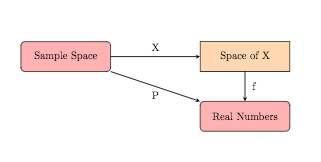
\includegraphics[width=1\linewidth]{images/randomvariable.png}
\typeout{************************************************}
\typeout{Section 4.7 Probability Functions}
\typeout{************************************************}
\section[Probability Functions]{Probability Functions}\label{ProbabilityFunctions}
In the formulas below, we will presume that we have a random variable X which maps the sample space S onto some range of real numbers R.  From this set, we then can define a probability function f(x) which acts on the numerical values in R and returns another real number.  We attempt to do so to obtain (for discrete values) P(sample space value s)\( = f(X(s))\).  That is, the probability of a given outcome s is equal to the composition which takes s to a numerical value x which is then plugged into f to get the same final values.%
\begin{definition}[Probability Mass Function]\label{definition-27}
Given a discrete random variable X on a space R, a probability mass function on X is given by a function \(f:R \rightarrow \mathbb{R}\) such that:
		\begin{align*}
& \forall x \in R , f(x) \gt 0\\
& \sum_{x \in R} f(x) = 1\\
& A \subset R \Rightarrow P(X \in A) = \sum_{x \in A}f(x)
\end{align*}\end{definition}
\begin{definition}[Probability Density Function]\label{definition-28}
Given a continuous random variable X on a space R, a probability density function on X is given by a function \(f:R \rightarrow \mathbb{R}\) such that:
			\begin{align*}
& \forall x \in R , f(x) \gt 0\\
& \int_{R} f(x) = 1\\
& A \subset R \Rightarrow P(X \in A) = \int_{A} f(x) dx
\end{align*}\end{definition}
\begin{example}[Discrete Probability Function]\label{example-17}

	Consider \(f(x) = x/10\) over R = {1,2,3,4}.  Then, f(x) is obviously positive for each of the values in R and certainly \(\sum_{x \in R} f(x) = f(1) + f(2) + f(3) + f(4) = 1/10 + 2/10 + 3/10 + 4/10 = 1\). Therefore, f(x) is a probability mass function over the space R.
	%
\end{example}
\begin{lstlisting}[style=sageinput]
# Combining all of the above into one interactive cell
@interact
def _(D = input_box([1,2,3,5,6,8,9,11,12,14],label="Enter domain R (in brackets):"), 
       Probs = input_box([1/20,1/20,1/20,3/20,1/20,4/20,4/20,1/20,1/20,3/20],label="Enter corresponding f(x) (in brackets):"),
       n_samples=slider(100,10000,100,100,label="Number of times to sample from this distribution:")):
    n = len(D)
    R = range(n)
    one_huh = sum(Probs)
    pretty_print('\n\nJust to be certain, we should check to make certain the probabilities sum to 1\n')
    pretty_print(html('$\sum_{x\epsilon R} f(x) = %s$'%str(one_huh)))
    
    G = Graphics()
    if len(D)==len(Probs):
        f = zip(D,Probs)
        meanf = 0
        variancef = 0
        for k in R:
            meanf += D[k]*Probs[k]
            variancef += D[k]^2*Probs[k]
            G += line([(D[k],0),(D[k],Probs[k])],color='green')
        variancef = variancef - meanf^2
        sd = sqrt(variancef)
        G += points(f,color='blue',size=50)
        G += point((meanf,0),color='yellow',size=60,zorder=3)
        G += line([(meanf-sd,0),(meanf+sd,0)],color='red',thickness=5)
    
        g = DiscreteProbabilitySpace(D,Probs)
        pretty_print('     mean = %s'%str(meanf))
        pretty_print(' variance = %s'%str(variancef))
    
        #  perhaps to add mean and variance for pmf here
    else:
        print 'Domain D and Probabilities Probs must be lists of the same size'
    
    #  Now, let's sample from the distribution given above and see how a random sampling matches up

    counts = [0] * len(Probs)
    X = GeneralDiscreteDistribution(Probs)
    sample = []

    for _ in range(n_samples):
        elem = X.get_random_element()
        sample.append(D[elem])
        counts[elem] += 1
    Empirical = [1.0*x/n_samples for x in counts] # random
    
    samplemean = mean(sample)
    samplevariance = variance(sample)
    sampdev = sqrt(samplevariance)
    
    E = points(zip(D,Empirical),color='orange',size=40)
    E += point((samplemean,0.005),color='brown',size=60,zorder=3)
    E += line([(samplemean-sampdev,0.005),(samplemean+sampdev,0.005)],color='orange',thickness=5)    
    (G+E).show(ymin=0,figsize=(8,5))
\end{lstlisting}
\begin{example}[Continuous Probability Function]\label{example-18}

	Consider \(f(x) = x^2/c\) for some positive real number c and presume R = [-1,2]. Then f(x) is nonnegative (and only equals zero at one point). To make f(x) a probability density function, we must have
	\begin{equation*}\int_{x \in R} f(x) = 1.\end{equation*}
	In this instance you get
	\begin{equation*}1 = \int_{-1}^2 x^2/c = x^3/(3c) |_{-1}^2 = \frac{8}{3c} - \frac{-1}{3c} = \frac{3}{c}\end{equation*}
	Therefore, f(x) is a probability density function over R provided   = 3.
	%
\end{example}
\begin{definition}[Distribution Function]\label{definition-29}
Given a random variable X on a space R, a probability distribution function on X is given by a function 
				   \(F:\mathbb{R} \rightarrow \mathbb{R}\) such that \(\displaystyle F(x)=P(X \le x)\)\end{definition}
\begin{example}[Discrete Distribution Function]\label{example-19}
Using \(f(x) = x/10\) over R = {1,2,3,4} again, note that F(x) will only change at these four domain values. We get
	
	\leavevmode%
\begin{table}
\centering
\begin{tabular}{rr}
X&F(x)\tabularnewline\hrulemedium
\(x \lt 1\)&0\tabularnewline[0pt]
\(1 \le x \lt 2\)&1/10\tabularnewline[0pt]
\(2 \le x \lt 3\)&3/10\tabularnewline[0pt]
\(3 \le x \lt 4\)&6/10\tabularnewline[0pt]
\(4 \le x \)&1
\end{tabular}
\end{table}

	%
\end{example}
\begin{example}[Continuous Distribution Function]\label{example-20}

	Consider \(f(x) = x^2/3\) over R = [-1,2].  Then, for \(-1 \le x \le 2\),
	\begin{equation*}F(x) = \int_{-1}^x u^2/3 du = x^3/9 + 1/9.\end{equation*}
	Notice, F(-1) = 0 since nothing has yet been accumulated over values smaller than -1 and F(2)=1 since by that time everything has been accumulated. In summary:
	
	\leavevmode%
\begin{table}
\centering
\begin{tabular}{rr}
X&F(x)\tabularnewline\hrulemedium
\(x \lt -1\)&0\tabularnewline[0pt]
\(-1 \le x \lt 2\)&\(x^3/9 + 1/9\)\tabularnewline[0pt]
\(2 \le x\)&1
\end{tabular}
\end{table}

	
	
	%
\end{example}
\typeout{************************************************}
\typeout{Section 4.8 Properties of the Distribution Function}
\typeout{************************************************}
\section[Properties of the Distribution Function]{Properties of the Distribution Function}\label{section-24}
\begin{theorem}[]\label{theorem-Fmin}
\(F(x)=0, \forall x \le \inf(R)\)\end{theorem}
\begin{proof}\hypertarget{proof-19}{}
\end{proof}
\begin{theorem}[]\label{theorem-Fmax}
\(F(x)=1, \forall x \ge \sup(R)\)\end{theorem}
\begin{proof}\hypertarget{proof-20}{}
\end{proof}
\begin{theorem}[]\label{theorem-26}
F is non-decreasing\end{theorem}
\begin{proof}\hypertarget{proof-21}{}
Case 1: R discrete%
\begin{align*}
\forall x_1,x_2 \in \mathbb{Z} \ni x_1 \lt x_2\\
F(x_2) & = \sum_{x \le x_2} f(x) \\
& = \sum_{x \le x_1} f(x) + \sum_{x_1 \lt x \le x_2} f(x)\\
& \ge \sum_{x \le x_1} f(x) = F(x_1)
\end{align*}\par
Case 2: R continuous%
\begin{align*}
\forall x_1,x_2 \in \mathbb{R} \ni x_1 \lt x_2\\
F(x_2) & = \int_{-\infty}^{x_2} f(x) dx \\
 & = \int_{-\infty}^{x_1} f(x) dx + \int_{x_1}^{x_2} f(x) dx\\
 & \ge \int_{-\infty}^{x_1} f(x) dx\\
 & = F(x_1)
\end{align*}\end{proof}
\begin{theorem}[Using Discrete Distribution Function to compute probabilities]\label{theorem-Fvsf-discrete}
for \(x \in R, f(x) = F(x) - F(x-1)\)\end{theorem}
\begin{theorem}[Using Continuous Distribution function to compute probabilities]\label{theorem-Fvsf-continuyous}
for \(a \lt b, (a,b) \in R, P(a \lt X \lt b) = F(b) - F(a)\)\end{theorem}
\begin{corollary}[]\label{corollary-ProbPointZero-continuous}
For continuous distributions, P(X = a) = 0\end{corollary}
\typeout{************************************************}
\typeout{Section 4.9 Standard Units}
\typeout{************************************************}
\section[Standard Units]{Standard Units}\label{section-25}
Any distribution variable can be converted to “standard units” using the linear translation 
			\(\displaystyle z = \frac{x-\mu}{\sigma}\). In doing so, then values of z will always represent the number of
			standard deviations x is from the mean and will provide “dimensionless” comparisons.%
\typeout{************************************************}
\typeout{Section 4.10 Expected Value}
\typeout{************************************************}
\section[Expected Value]{Expected Value}\label{section-26}
Blaise Pascal was a 	17th century mathematician and philosopher who was accomplished in many areas but may likely be best known to you for his creation of what is now known as Pascal's Triangle. As part of his philosophical pursuits, he proposed what is known as "Pascal's wager". It suggests two  mutually exclusive outcomes: that God exists or that he does not. His argument is that a rational person should live as though God exists and seek to believe in God. If God does not actually exist, such a person will have only a finite loss (some pleasures, luxury, etc.), whereas they stand to receive infinite gains as represented by eternity in Heaven and avoid an infinite losses of eternity in Hell. This type of reasoning is part of what is known as "decision theory".
	%
\par
You may not confront such dire payouts when making your daily decisions but we need a formal method for making these determinations precise. The procedure for doing so is what we call expected value.
	%
\begin{definition}[Expected Value]\label{definition-30}
Given a random variable X over space R, corresponding probability function f(x) and "value function" u(x), the expected value of u(x) is given by
	\begin{equation*}E = E[u(X)] = \sum_{x \in R} u(x) f(x)\end{equation*}
	provided X is discrete, or
	\begin{equation*}E = E[u(X)] = \int_R u(x)f(x) dx\end{equation*}
	provided X is continuous.
	%
\end{definition}
\begin{example}[Discrete Expected Value]\label{example-21}
Consider \(f(x) = x/10\) over R = {1,2,3,4} where the payout is 10 euros if x=1, 5 euros if x=2, 2 euros if x=3 and -7 euros if x = 4.  Then your value function would be u(1)=10, u(2) = 5, u(3)=2, and u(4) = -7. Computing the expect payout gives
	\begin{equation*}E = 10 \times 1/10 + 5 \times 2/10 + 2 \times 3/10 - 7 \times 4/10 = -2/10\end{equation*}
	Therefore, the expected payout is actually negative due to a relatively large negative payout associated with the largest likelihood outcome and the larger positive payout only associated with the least likely outcome.
	%
\end{example}
\begin{example}[Continuous Expected Value]\label{example-22}

	Consider \(f(x) = x^2/3\) over R = [-1,2] with value function given by \(u(x) = e^x - 1\). Then, the expected value for u(x) is given by
	\begin{equation*}E = \int_{-1}^2 (e^x-1) \cdot x^2/3 = -1/9 \cdot (e + 15) \cdot e^{-1} + 2/3 \cdot e^2 - 8/9 \approx 3.3129\end{equation*}
	%
\end{example}
\par
So, going back to Pascal's wager, let X = 0 represent disbelief when God doesn't exist and X = 1 represent disbelief when God does exist, X = 2 represent belief when God does exist, and X = 3 represent belief when God does not exist. Let p be the likelihood that God exists. Then you can compute the expected value of disbelief and the expect value of belief by first creating a value function. Below, for argument sake we are somewhat randomly assign a value of one million to disbelief if God doesn't exist. The conclusions are the same if you choose any other finite number...
	\begin{gather*}
u(0) = 1,000,000, f(0) = 1-p\\
u(1) = -\infty, f(1) = p\\
u(2) = \infty, f(2) = p\\
u(3) = 0, f(3) = 1-p
\end{gather*}
	Then, 
	\begin{align*}
E[disbelief] & = u(0)f(0) + u(1)f(1)\\
& = 1000000 \times (1-p) - \infty \times p\\
& = -\infty
\end{align*}
	if p>0. On the other hand, 
	\begin{align*}
E[belief] & = u(2)f(2) + u(3)f(3)\\
& = \infty \times p + 0 \times (1-p)\\
& = \infty
\end{align*}
	if p>0. So Pascal's conclusion is that if there is even the slightest chance that God exists then belief is the smart and scientific choice.
	%
\typeout{************************************************}
\typeout{Chapter 5 Binomial, Geometric, and Negative Binomial Distributions}
\typeout{************************************************}
\chapter[Binomial, Geometric, and Negative Binomial Distributions]{Binomial, Geometric, and Negative Binomial Distributions}\label{BinomNegBinom}
\typeout{************************************************}
\typeout{Introduction  }
\typeout{************************************************}
Distributions relating number of successes to number of trials with one 
	of these variable and the other fixed.%
\typeout{************************************************}
\typeout{Section 5.1 Binomial Distribution}
\typeout{************************************************}
\section[Binomial Distribution]{Binomial Distribution}\label{BinomialDistribution}
Consider the situation where one can observe a sequence  of n
	independent trials with the likelihood of a 
	success on each individual trial stays constant from trial to trial.
	Call this likelihood the probably of "success" and 
	denote its value by 
	\(p\) where \( 0 \lt p \lt 1 \).  
	If we let the variable \(X\) measure the number of successes 
	obtained when doing a fixed number of trials n, then the resulting
	distribution of probabilities is called a Binomial Distribution.%
\typeout{************************************************}
\typeout{Subsection 5.1.1 Derivation of Binomial Probability Function}
\typeout{************************************************}
\subsection[Derivation of Binomial Probability Function]{Derivation of Binomial Probability Function}\label{subsection-11}
 Since successive trials are independent, then the probability of X successes occurring within n 
		trials is given by 
		\(P(X=x) = \binom{n}{x}P(SS...SFF...F) = \binom{n}{x}p^x(1-p)^{n-x}\)%
\typeout{************************************************}
\typeout{Subsection 5.1.2 Binomial Distribution mean}
\typeout{************************************************}
\subsection[Binomial Distribution mean]{Binomial Distribution mean}\label{subsection-12}
\begin{align*}
 \mu = E[X] & = \sum_{x=0}^{n} {x \binom{n}{x} p^x (1-p)^{n-x}}\\
 & = \sum_{x=1}^{n} {x \frac{n(n-1)!}{x(x-1)!(n-x)!} p^x (1-p)^{n-x}}\\
 & = np \sum_{x=1}^{n} {\frac{(n-1)!}{(x-1)!((n-1)-(x-1))!} p^{x-1} (1-p)^{(n-1)-(x-1)}}
\end{align*}Using the change of variables \(k=x-1\) and \(m = n-1\) yields a binomial series%
\begin{align*}
 & = np \sum_{k=0}^{m} {\frac{m!}{k!(m-k)!} p^k (1-p)^{m-k}}\\
 & = np (p + (1-p))^m = np
\end{align*}\typeout{************************************************}
\typeout{Subsection 5.1.3 Binomial Distribution variance}
\typeout{************************************************}
\subsection[Binomial Distribution variance]{Binomial Distribution variance}\label{subsection-13}
\begin{align*}
 \sigma^2 = E[X(X-1)] + \mu - \mu^2 & = \sum_{x=0}^{n} {x(x-1) \binom{n}{x} p^x (1-p)^{n-x}} + np - n^2p^2\\
 & = \sum_{x=2}^{n} {x(x-1) \frac{n(n-1)(n-2)!}{x(x-1)(x-2)!(n-x)!} p^x (1-p)^{n-x}}  + np - n^2p^2\\
 & = n(n-1)p^2 \sum_{x=2}^{n} {\frac{(n-2)!}{(x-2)!((n-2)-(x-2))!} p^{x-2} (1-p)^{(n-2)-(x-2)}} + np - n^2p^2
\end{align*}Using the change of variables \(k=x-2\) and \(m = n-2\) yields a binomial series%
\begin{align*}
 & = n(n-1)p^2  \sum{k=0}^{m} {\frac{m!}{k!(m-k)!} p^k (1-p)^{m-k}} + np - n^2p^2\\
 & = n(n-1)p^2 + np - n^2p^2 = np - np^2 = np(1-p)
\end{align*}\typeout{************************************************}
\typeout{Section 5.2 Geometric Distribution}
\typeout{************************************************}
\section[Geometric Distribution]{Geometric Distribution}\label{GeometricDistribution}
Consider the situation where one can observe a sequence  of independent
	trials where the likelihood of a success on each individual trial
	stays constant from trial to trial. Call this likelihood the probably of
	"success" and denote its value by \(p\) 
	where \( 0 \lt p \lt 1 \).  
	If we let the variable \(X\) measure the number of trials needed in order
	to obtain the first success, 
	then the resulting distribution of probabilities is called a 
	Geometric Distribution.%
\typeout{************************************************}
\typeout{Subsection 5.2.1 Derivation of Geometric Probability Function}
\typeout{************************************************}
\subsection[Derivation of Geometric Probability Function]{Derivation of Geometric Probability Function}\label{subsection-14}
 Since successive trials are independent, then the probability 
			of the first success occurring on the mth trial presumes that
			the previous m-1 trials were all failures.  Therefore the 
			desired probability is given by %
\begin{equation*}f(x) = P(X=m) = P(FF...FS) = (1-p)^{m-1}p\end{equation*}\typeout{************************************************}
\typeout{Subsection 5.2.2 Properties of the Geometric DistributionGeometric Distribution sums to 1}
\typeout{************************************************}
\subsection[Properties of the Geometric DistributionGeometric Distribution sums to 1]{Properties of the Geometric DistributionGeometric Distribution sums to 1}\label{subsection-15}
\begin{gather*}
\SUM {k=1} {\infty} {f(x)} = \sum_{k=1}^{\infty} {(1-p)^{k-1} p} = p \sum_{j=0}^{\infty} {(1-p)^j} = p \frac{1}{1-(1-p)} = 1
\end{gather*}\typeout{************************************************}
\typeout{Subsection 5.2.3 Derivation of Geometric Mean}
\typeout{************************************************}
\subsection[Derivation of Geometric Mean]{Derivation of Geometric Mean}\label{subsection-16}
 %
\begin{align*}
\mu & = E[X] = \sum_{k=0}^{\infty} {k(1-p)^{k-1}p}\\
 & = p \sum_{k=1}^{\infty} {k(1-p)^{k-1}}\\
 & = p \frac{1}{(1-(1-p))^2}\\
 & = p \frac{1}{p^2} = \frac{1}{p}
\end{align*}\typeout{************************************************}
\typeout{Subsection 5.2.4 Derivation of Geometric Variance}
\typeout{************************************************}
\subsection[Derivation of Geometric Variance]{Derivation of Geometric Variance}\label{subsection-17}
 %
\begin{align*}
\sigma^2 & = E[X(X-1)] + \mu - \mu^2 \\
 & = \su _{k=0}^{\infty} {k(k-1)(1-p)^{k-1}p} + \mu - \mu^2 \\
 & = (1-p)p \sum_{k=2}^{\infty} {k(k-1)(1-p)^{k-2}} + \frac{1}{p} - \frac{1}{p^2}\\
 & = (1-p)p \frac{2}{(1-(1-p))^3} + \frac{1}{p} - \frac{1}{p^2}\\
 & = \frac{1-p}{p^2}
\end{align*}\typeout{************************************************}
\typeout{Subsection 5.2.5 Derivation of Geometric Distribution Function}
\typeout{************************************************}
\subsection[Derivation of Geometric Distribution Function]{Derivation of Geometric Distribution Function}\label{subsection-18}
 Consider the accumulated probabilities over a range of values...%
\begin{align*}
 P(X \le a) & = 1 - P(X \gt a)\\
 & = 1- \sum_{k={a+1}}^{\infty} {(1-p)^{k-1}p}\\
 & = 1- p \frac{(1-p)^{a}}{1-(1-p)}\\
 & = 1- (1-p)^{a}
\end{align*}\typeout{************************************************}
\typeout{Section 5.3 Negative Binomial}
\typeout{************************************************}
\section[Negative Binomial]{Negative Binomial}\label{section-29}
Consider the situation where one can observe a sequence  of independent
	trials where the likelihood of a success on each individual trial
	stays constant from trial to trial. Call this likelihood the probably of
	"success" and denote its value by \(p\) 
	where \( 0 \lt p \lt 1 \).  
	If we let the variable \(X\) measure the number of trials needed in order
	to obtain the rth success, \(r \ge 1\) 
	then the resulting distribution of probabilities is called a 
	Geometric Distribution.%
\par
Note that r=1 gives the Geometric Distribution.%
\typeout{************************************************}
\typeout{Subsection 5.3.1 Negative Binomial Series}
\typeout{************************************************}
\subsection[Negative Binomial Series]{Negative Binomial Series}\label{subsection-19}
\begin{theorem}[]\label{theorem-NegBinomSeries}
\(\displaystyle \frac{1}{(a+b)^n} = \sum_{k=0}^{\infty} {(-1)^k \binom{n + k - 1}{k} a^k b^{-n-k}}\)\end{theorem}
\begin{proof}\hypertarget{proof-22}{}
First, convert the problem to a slightly different form:%
\( \frac{1}{(a+b)^n} = \frac{1}{b^n} \frac{1}{(\frac{a}{b}+1)^n} 
						 = \frac{1}{b^n} \sum_{k=0}^{\infty} {(-1)^k \binom{n + k - 1}{k} \left ( \frac{a}{b} \right ) ^k}
			\)\par
So, let's replace \(\frac{a}{b} = x\) and ignore for a while the term factored out. Then, we only need to show %
\begin{gather*}
\sum_{k=0}^{\infty} {(-1)^k \binom{n + k - 1}{k} x^k} = \left ( \frac{1}{1+x} \right )^n 
\end{gather*}\par
However%
\begin{align*}
 \left ( \frac{1}{1+x} \right )^n & = \left ( \frac{1}{1 - (-x)} \right )^n \\
 & = \left ( \sum_{k=0}^{\infty} {(-1)^k x^k} \right )^n
\end{align*}\par
This infinite sum raised to a power can be expanded by distributing terms in the standard way. 
			In doing so, the various powers of x multiplied together
			will create a series in powers of x involving \(x^0, x^1, x^2, ...\).  
			To detemine the final coefficients notice that the number of time \(m^k\) will 
			appear in this product depends upon the number of ways one can write k as a sum of nonnegative integers.%
\par
For example, the coefficient of \(x^3\) will come from the n ways of multiplying the coefficients 
			\(x^3, x^0, ..., x^0\) and \(x^2, x^1, x^0, ..., x^0\)
			 and \(x^1, x^1, x^1, x^0,..., x^0\). This is equivalent to finding the number of ways to write the 
			 number k as a sum of nonnegative integers. The possible set of
			 nonnegative integers is {0,1,2,...,k} and one way to count the combinations is to separate k *'s by n-1 |'s.  
			 For example, if k = 3 then *||** means 
			 \(x^1 x^0 x^2 = x^3\). Similarly for k = 5 and |**|*|**| implies \( x^0 x^2 x^1 x^2 x^0 = x^5\). 
			 The number of ways to interchange the identical *'s among the
			 idential |'s is \(\binom{n+k-1}{k}\). %
\par
Furthermore, to obtain an even power of x will require an even number of odd powers and an odd power of x 
			 will require an odd number of odd powers. So, the 
			 coefficient of the odd terms stays odd and the coefficient of the even terms remains even. Therefore,%
\begin{gather*}
 \left ( \frac{1}{1+x} \right )^n = \sum_{k=0}^{\infty} {(-1)^k \binom{n + k - 1}{k} x^k}
\end{gather*}\par
Similarly,%
\( \left ( \frac{1}{1-x} \right )^n = \left ( \sum_{k=0}^{\infty} {x^k} \right )^n = \sum_{k=0}^{\infty} {\binom{n + k - 1}{k} x^k}\)\end{proof}
\typeout{************************************************}
\typeout{Subsection 5.3.2 Negative Binomial Distribution FormulasNegative Binomial Distribution Sums to 1}
\typeout{************************************************}
\subsection[Negative Binomial Distribution FormulasNegative Binomial Distribution Sums to 1]{Negative Binomial Distribution FormulasNegative Binomial Distribution Sums to 1}\label{subsection-20}
Consider the situation where one can observe a sequence  of independent trials with the likelihood of a success 
		on each individual trial \(p\) where 
		\( 0 \lt p \lt 1 \).  For a positive integer r, let the variable \(X\) measure the number of 
		trials needed in order to obtain the rth success.
		Then the resulting distribution of probabilities is called a Negative Binomial Distribution.%
\par
 Since successive trials are independent, then the probability of the rth success occurring on the 
			mth trial presumes that in 
			the previous m-1 trials were r-1 successes and m-r failures.  Therefore the desired probability is given by 
			\begin{gather*}
P(X=m) = \binom{m - 1}{r-1}(1-p)^{m-r}p^r
\end{gather*}
			%
\(\SUM {m=r} {\infty} {\binom{m - 1}{r-1}(1-p)^{m-r}p^r} & = p^r \SUM {m=r} {\infty} {\binom{m - 1}{r-1}(1-p)^{m-r}}\)\par
and by using \(k = m-r\)%
\begin{align*}
 & = p^r \sum_{k=0}^{\infty} {\binom{r + k - 1}{k}(1-p)^k}\\
 & = p^r \frac{1}{(1-(1-p))^r}\\
 & = 1
\end{align*}\typeout{************************************************}
\typeout{Chapter 6 Poisson, Exponential, and Gamma Distributions}
\typeout{************************************************}
\chapter[Poisson, Exponential, and Gamma Distributions]{Poisson, Exponential, and Gamma Distributions}\label{PoissonExponential}
\typeout{************************************************}
\typeout{Section 6.1 Poisson Distribution}
\typeout{************************************************}
\section[Poisson Distribution]{Poisson Distribution}\label{section-30}
\typeout{************************************************}
\typeout{Section 6.2 Exponential Distribution}
\typeout{************************************************}
\section[Exponential Distribution]{Exponential Distribution}\label{section-31}
\typeout{************************************************}
\typeout{Section 6.3 Gamma Distribution}
\typeout{************************************************}
\section[Gamma Distribution]{Gamma Distribution}\label{section-32}
\typeout{************************************************}
\typeout{Chapter 7 Normal Distributions}
\typeout{************************************************}
\chapter[Normal Distributions]{Normal Distributions}\label{Normal}
\typeout{************************************************}
\typeout{Section 7.1 Properties of the Normal Distribution}
\typeout{************************************************}
\section[Properties of the Normal Distribution]{Properties of the Normal Distribution}\label{section-33}

	You have seen that most distributions become "bell shaped" as certain parameters are allowed to increase. The question might arise regarding whether this always must happen or is it just a happy coincidence. The amazing answer is that if you interpret the question in the correct way then this is always true.%

	\begin{definition}[The Normal Distribution]\label{definition-31}
Given two parameters \(\mu\) and \(\sigma\) a random variable X with density function
	\begin{equation*}
	f(x) = \frac{1}{\sigma \sqrt{2 \pi}} e^{ \left ( \frac{x-\mu}{\sigma} \right ) ^2 / 2}
	\end{equation*}\end{definition}
\begin{theorem}[]\label{theorem-30}

	If \(\mu =0\) and \(\sigma=1\), then we say X has a standard normal distribution and often use Z as the variable name. In this case, the density function reduces to
	\begin{equation*}
	f(x) = \frac{1}{\sqrt{2 \pi}} e^{ z^2 / 2}
	\end{equation*}\end{theorem}
\begin{proof}\hypertarget{proof-23}{}
Convert to "standard units" using the conversion \(z = \frac{x-\mu}{\sigma} = \frac{x-0}{1} = x\).%
\end{proof}
\typeout{************************************************}
\typeout{Section 7.2 Theorems}
\typeout{************************************************}
\section[Theorems]{Theorems}\label{section-34}
\typeout{************************************************}
\typeout{Section 7.3 Chi-Square Distribution}
\typeout{************************************************}
\section[Chi-Square Distribution]{Chi-Square Distribution}\label{section-35}
\typeout{************************************************}
\typeout{Section 7.4 Central Limit Theorem}
\typeout{************************************************}
\section[Central Limit Theorem]{Central Limit Theorem}\label{section-36}

Often, when one wants to solve various scientific problems, several assumptions will be made regarding the nature of the underlying setting and base their conclusions on those assumptions.  Indeed, if one is going to use a Binomial Distribution or a Negative Binomial Distribution, an assumption on the value of p is necessary.  For Poisson and Exponential Distributions, one must know the mean.  For Normal Distributions, one must assume values for both the mean and the standard deviation.   Where do these values come from?  Often, one may perform a preliminary study and obtain a sample statistic...such as a sample mean or a relative frequency and use these values for μ or p.%
\par

But what is the underlying distribution of these sample statistics?  The Central Limit Theorem gives the answer...%
\par
To motivate this discussion, consider the following two interactive experiments.  For the first graph below, a sequence of N random samples, each of size r, ranging from 0 to "Range" is generated and graphed as small data points.  As the number of samples N and the sample size r increase, notice that the data seems to cover the entire range of possible values relatively uniformly.  (For this scatter plot note that each row represents the data for one sample of size r.  The larger the N, the greater the number of rows.)  Each row is averaged and that mean value is plotted on the graph as a red circle.  If you check the "Show_Mean" box, the mean of these circles is indicated by the green line in the middle of the plot.
%
\par

For the second graph below, the means are collected and the relative frequency of each is plotted.  As N increases, you should see that the results begin to show an interesting tendency.   As you increase the data range, you may notice this graph has a larger number of data values.  Smoothing groups this data into intervals of length two for perhaps a graph with less variability.
%
\par

Consider each of the following:
\leavevmode%
\begin{itemize}[label=\textbullet]
\item{}
As N increases with single digit values of r, what appears to happen to the mean and range of the means?  How does increasing the data range from 1-100 to 1-200 or 1-300 affect these results?%
\item{}As N increases (say, for a middle value of r), what appears to happen to the means?  How does increasing the data range from 1-100 to 1-200 or 1-300 affect these results?%
\item{}As r increases (say, for a middle value of N), what appears to happen to the range of the averages?  Does your conclusion actually depend upon the value of N?  (Look at the graph and don't worry about the actual numerical values.)
How does increasing N for the second graph affect the skewness and kurtosis of that graph?  Do things change significantly as r is increased?  %
\end{itemize}

%
\begin{lstlisting}[style=sageinput]
var('n,k')
from sage.finance.time_series import TimeSeries

@interact(layout=dict(top=[['Range'],['Show_Mean', 'Smoothing']],  
bottom=[['N'],['r']]))

def _(Range=[100,200,300,500],N=slider(5,200,2,2,label="N = Number of Samples"),r=slider(3,200,1,2,label="r = Sample Size"),Show_Mean=False,Smoothing=False):
    R=[1..N]     #  R ranges over the number of samples...will point to the list of averages
    rangemax = Range

    data = random_matrix(ZZ,N,r,x=rangemax)
    datapoints = []
    avg_values = []
    avg_string = []
    averages = []
    for n in range(N):
        temp = 0
        for k in range(r):
            datapoints += [(data[n][k],n)]
            temp += data[n][k]
        avg_values.append(round(temp/r))
        if Smoothing:
            avg_string.append(str(2*round((temp/r)/2)))    
        else:
            avg_string.append(str(round(temp/r)))
            
        averages += [(round(temp/r),n)]   #  make these averages integers for use in grouping later
    SCAT = scatter_plot(datapoints,markersize=2,edgecolor='red',figsize=(10,4),axes_labels=['Sample Values','Sample Number'])
    AVGS = scatter_plot(averages,markersize=50,edgecolor='blue',marker='o',figsize=(7,4))
    
    freqslist = frequency_distribution(avg_string,1).function().items()
       
       
# compute sample statistics for the raw data as well as for the N averages
    Mean_data = (sum(sum(data))/(N*r)).n()
#    STD_data = sqrt(sum(sum( (data-Mean_data)^2 ))/(N*r)).n()
    Mean_averages = mean(avg_values).n()
#    STD_averages = sqrt(variance(avg_values).n())
#    print "Data mean =",Mean_data," vs Mean of the averages =",Mean_averages
#    print "Data STD = ",STD_data," vs Standard Dev of avgs =", STD_averages
    if Show_Mean:
        avg_line = line([(Mean_data,0),(Mean_data,N-1)],rgbcolor='green',thickness=10)
        avg_text = text('xbar',(Mean_data,N),horizontal_alignment='right',rgbcolor='green')
    else:
        avg_line = Graphics()
        avg_text = Graphics()
            
#  Plot a scatter plot exhibiting uniformly random data and the collection of averages 
    print(html("The random data plot on the left with each row representing a sample with size determined by\n"+
         "the slider above and each circle representing the average for that particular sample.\n"+
         "First, keep sample size relatively low and increase the number of samples.  Then, \n"+
         "watch what happens when you slowly increase the sample size."))

    
#  Plot the relative frequencies of the grouped sample averages
    print(html("Now, the averages (ie. the circles) from above are collected and counted\n"+
         "with the relative frequency of each average graphed below.  For a relatively large number of\n"+
         "samples, notice what seems to happen to these averages as the sample size increases."))
    if Smoothing:
        binRange = Range//2
    else:
        binRange = Range
    
    # normed=True  # if you want to have relative frequencies below
    
    his_low = 2*rangemax/7
    his_high = 5*rangemax/7
    
    T = histogram(avg_values,normed=False,bins=binRange,range=(his_low,his_high),axes_labels=['Sample Averages','Frequency']) 
    #T = TimeSeries(avg_values).plot_histogram(axes_labels=['Sample Averages','Frequency'])   
    
    pretty_print('Scatter Plot of random data.  Horizontal is number of samples.')
    (SCAT+AVGS+avg_line+avg_text).show()
    pretty_print('Histogram of Sample Averages')
    T.show(figsize=(5,2))
\end{lstlisting}
\begin{lstlisting}[style=sageinput]
var('n,k')
from sage.finance.time_series import TimeSeries

@interact(layout=dict(top=[['Range'],['Show_Mean', 'Smoothing']],  
bottom=[['N'],['r']]))

def _(Range=[100,200,300,500],N=slider(5,200,2,2,label="N = Number of Samples"),r=slider(3,200,1,2,label="r = Sample Size"),Show_Mean=False,Smoothing=False):
    R=[1..N]     #  R ranges over the number of samples...will point to the list of averages
    rangemax = Range

    data = random_matrix(ZZ,N,r,x=rangemax)
    datapoints = []
    avg_values = []
    avg_string = []
    averages = []
    for n in range(N):
        temp = 0
        for k in range(r):
            datapoints += [(data[n][k],n)]
            temp += data[n][k]
        avg_values.append(round(temp/r))
        if Smoothing:
            avg_string.append(str(2*round((temp/r)/2)))    
        else:
            avg_string.append(str(round(temp/r)))
            
        averages += [(round(temp/r),n)]   #  make these averages integers for use in grouping later
    SCAT = scatter_plot(datapoints,markersize=2,edgecolor='red',figsize=(10,4),axes_labels=['Sample Values','Sample Number'])
    AVGS = scatter_plot(averages,markersize=50,edgecolor='blue',marker='o',figsize=(7,4))
    
    freqslist = frequency_distribution(avg_string,1).function().items()
       
       
# compute sample statistics for the raw data as well as for the N averages
    Mean_data = (sum(sum(data))/(N*r)).n()
#    STD_data = sqrt(sum(sum( (data-Mean_data)^2 ))/(N*r)).n()
    Mean_averages = mean(avg_values).n()
#    STD_averages = sqrt(variance(avg_values).n())
#    print "Data mean =",Mean_data," vs Mean of the averages =",Mean_averages
#    print "Data STD = ",STD_data," vs Standard Dev of avgs =", STD_averages
    if Show_Mean:
        avg_line = line([(Mean_data,0),(Mean_data,N-1)],rgbcolor='green',thickness=10)
        avg_text = text('xbar',(Mean_data,N),horizontal_alignment='right',rgbcolor='green')
    else:
        avg_line = Graphics()
        avg_text = Graphics()
            
#  Plot a scatter plot exhibiting uniformly random data and the collection of averages 
    print(html("The random data plot on the left with each row representing a sample with size determined by\n"+
         "the slider above and each circle representing the average for that particular sample.\n"+
         "First, keep sample size relatively low and increase the number of samples.  Then, \n"+
         "watch what happens when you slowly increase the sample size."))

    
#  Plot the relative frequencies of the grouped sample averages
    print(html("Now, the averages (ie. the circles) from above are collected and counted\n"+
         "with the relative frequency of each average graphed below.  For a relatively large number of\n"+
         "samples, notice what seems to happen to these averages as the sample size increases."))
    if Smoothing:
        binRange = Range//2
    else:
        binRange = Range
    
    # normed=True  # if you want to have relative frequencies below
    
    his_low = 2*rangemax/7
    his_high = 5*rangemax/7
    
    T = histogram(avg_values,normed=False,bins=binRange,range=(his_low,his_high),axes_labels=['Sample Averages','Frequency']) 
    #T = TimeSeries(avg_values).plot_histogram(axes_labels=['Sample Averages','Frequency'])   
    
    pretty_print('Scatter Plot of random data.  Horizontal is number of samples.')
    (SCAT+AVGS+avg_line+avg_text).show()
    pretty_print('Histogram of Sample Averages')
    T.show(figsize=(5,2))
\end{lstlisting}
\typeout{************************************************}
\typeout{Subsection 7.4.1 }
\typeout{************************************************}
\subsection[]{}\label{subsection-21}

	Theorem
	%
\typeout{************************************************}
\typeout{Subsection 7.4.2 }
\typeout{************************************************}
\subsection[]{}\label{subsection-22}

	Approximating distributions
	Limiting distributions
	%
\typeout{************************************************}
\typeout{Chapter 8 Estimating Data using Intervals}
\typeout{************************************************}
\chapter[Estimating Data using Intervals]{Estimating Data using Intervals}\label{IntervalEstimation}
\typeout{************************************************}
\typeout{Section 8.1 Chebyshev}
\typeout{************************************************}
\section[Chebyshev]{Chebyshev}\label{section-37}
An interval centered on the mean in which at least a certain proportion
	of the actual data must lie.
	%
\begin{theorem}[Chebyshev's Theorem]\label{theorem-31}

	Given a random variable X with given mean μ and standard deviation σ, for k>1 at least
	2
	1 1
	k − of the observations lie within k standard deviations from the mean.
	\end{theorem}
\typeout{************************************************}
\typeout{Section 8.2 Measures of Spread}
\typeout{************************************************}
\section[Measures of Spread]{Measures of Spread}\label{section-38}
Measures of spread:
• Average Deviation from the Mean – always zero for any distribution
• Average Absolute Deviation from the Mean – difficult to deal with algebra when absolute values are used
• Average Squared Deviation from the Mean – always non-negative and good with algebra and calculus 
%
\begin{definition}[Variance]\label{definition-32}
The variance is a measure of spread found by using the average squared deviation from the mean
σ2
 = ( ) )(
2
1
k
n
k
k ∑ xfx =
− μ
if this value exists and is also denoted by Var(X). The positive square root of the variance is called the standard deviation
and is denoted by σ. \end{definition}
\end{document}